\documentclass[a4paper,10pt]{article}

\usepackage{color}
\usepackage{xcolor}
\usepackage{tikz}
\usepackage{amsmath}
\usepackage{amssymb}
\usepackage{amsthm}
\usepackage{graphicx}
\usepackage{mathtools}
\usepackage{wrapfig}
\usepackage{multirow}
\usepackage{comment}
\usepackage{natbib}
%\usepackage{float}
\usepackage{appendix}
\usepackage{enumitem}
\usepackage{newfloat}
\usepackage{subcaption}
\usepackage[utf8]{inputenc}
\usepackage{floatrow}
\usepackage{bm}
\usepackage{hyperref}
\usepackage{tcolorbox}
\usepackage{chngcntr}

\usetikzlibrary{calc}
\usetikzlibrary{fit}
\usetikzlibrary{decorations.shapes,shapes.misc,calc, positioning, hobby, backgrounds}


\tikzset{decorate sep/.style 2 args=
{decorate,decoration={shape backgrounds,shape=circle,shape size=#1,shape sep=#2}}}

\tikzset{cross/.style={cross out, draw=black, minimum size=2*(#1-\pgflinewidth), inner sep=0pt, outer sep=0pt},
%default radius will be 1pt. 
cross/.default={1pt}}

%\DeclarePairedDelimiter{\floor}{\lfloor}{\rightfloor}
%\DeclarePairedDelimiter{\ceil}{\lceil}{\rceil}

\newcommand{\denominator}{\ensuremath{n+\sum\limits_{j=1}^{h} k_{j}}}
\newcommand{\halflength}{\ensuremath{\floor{\frac{m}{2}}}}
\newcommand{\floor}[1]{\left \lfloor #1 \right \rfloor}
\newcommand{\ceil}[1]{\left \lceil #1 \right \rceil}
\newcommand{\pospart}[1]{\left( #1 \right)_{+}}
\newcommand{\negpart}[1]{\left( #1 \right)_{-}}
\newcommand{\set}[2]{\left\{ #1 \, | \, #2 \right\}}
\DeclareMathOperator*{\argmin}{\arg\!\min}

\newtheorem{theorem}{Theorem}[section]
\newtheorem{corollary}[theorem]{Corollary}
\newtheorem{lemma}[theorem]{Lemma}

\theoremstyle{definition}
\newtheorem{definition}[theorem]{Definition}

\theoremstyle{definition}
\newtheorem{example}[theorem]{Example}
 
\theoremstyle{remark}
\newtheorem*{remark}{Remark}

\theoremstyle{definition}
\newtheorem*{note}{Note}

\DeclareFloatingEnvironment[fileext=los,
    listname={List of Example Figures},
    name=Example Figure,
    placement=tbhp,
    within=section,]{examplefigure}
    
\DeclareFloatingEnvironment[fileext=los,
    listname={List of myFigures},
    name=Figure,
    placement=tbhp,
    within=section,]{myfigure}
    
%\counterwithin{figure}{section}

\title{Second Year Report}
\date{\today}
\author{Thomas Lowbridge \\ School of Mathematical Sciences \\ University of Nottingham}

\bibliographystyle{unsrtnat}

\begin{document}

\pagestyle{empty}
{
  \renewcommand{\thispagestyle}[1]{}
  \maketitle
  \tableofcontents  
}
\clearpage
\pagestyle{plain}


\setlength{\parindent}{0pt}
\setlength{\parskip}{1em}

\newpage
\pagenumbering{arabic}


\section{Literature Review}
\subsection{Overview of Search games}

Due to the high dependency on graphical structure, we provide a comprehensive guide to graph definitions in Appendix \ref{Appendix:Graph Definitions}.

\subsection{Review of Strategic Patrolling games}
A patrolling game $G=G(Q,T,m)$ is a win-lose, zero-sum game between a maximizing patroller (often referred to as she) and a minimizing attacker (often referred to as he). The parameters of the game are:
\begin{itemize}
\item The graph $Q=(N,E)$ made of nodes, $N$ ($|N|=n$), joined by edges, $E$, which can be represented by an adjacency matrix, $A$.
\item The length of time over which the game takes place, the time-horizon $T$.
\item The length of time the attack takes to complete, the attack-time $m$.
\end{itemize}

Two forms of the game exist: the one-off game, which is played in a finite time interval $\mathcal{T}=\{0,1,...,T-1\}$ denoted using $G^{o}$; and the periodic game, which is played on the time circle $\mathcal{T}^*=\{0,1,...,T-1\}$ (with the asterisk representing arithmetic on the time circle taking place modulo $T$) denoted using $G^p$. We will assume that $T \geq m$ , otherwise it clear that all attacks will fail.

The pure strategies available to the patroller are called patrols, choosing a starting position and how to walk along the graph Q, $W:\mathcal{T} \rightarrow N$. With no restrictions in the one-off game, but the restriction that the edge $(W(T-1),W(0)) \in E$ in the periodic game (so that $W(T)=W(0)$). Let $$\mathcal{W}=\{ W \, | \, W:\mathcal{T} \rightarrow N \text{ s.t } (W(t),W(t+1)) \in E \text{ for } t=0,...,T-2  \} $$ be the set of all pure patrols in the one-off game (and similarly $\mathcal{W}^*$ in the periodic game). Let there be some ordering to the strategies $W_{k} \in \mathcal{W}$ (or $W_{k} \in \mathcal{W}^{*}$) for $k=1,...,|\mathcal{W}|$ (or $k=1,...,|\mathcal{W}^*|$ in the periodic game).

The pure strategies available to the attacker are pairs, $[i,I]$ for $i \in N$, called the attack node, and $I=\{ \tau,\tau+1,...,\tau+m-1 \} \subseteq \mathcal{T}$ (or $I \subseteq \mathcal{T}^*$ if periodic) called the attack interval (starting at time $\tau$). Let $\mathcal{A}=\{[i,I] \, | \, i \in N , I \subseteq \mathcal{T} \}$ be the set of all possible pure attacks. Let there be some ordering to the strategies $A_{k} \in \mathcal{A}$ for $k=1,...,|\mathcal{A}|$.

A patrol, $W$, intercepts the attack, $[i,I]$, if $i \in W(I)=\{W(\tau),W(\tau+1),...,W(\tau+m-1)\}$ and as our game is Win-Lose the pure payoff function is
$$P(W,[i,I])=\left\{ \begin{array}{l}
1 \text{  if  } i \in W(I) ,\\
0 \text{  if  } i \notin W(I) .\\
\end{array}\right.$$
A pure payoff matrix $\mathcal{P}=(P(W_{i},A_{j}))_{i \in \{ 1,...,|\mathcal{W}| \}, j \in \{ 1,...,|\mathcal{A}| \}}$ (with the change of $\mathcal{W}$ to $\mathcal{W}^*$ if in the periodic game) stores Win ($1$) or Lose ($0$) for each pair of pure strategies.

Let $\Pi_{W}$ be the set of mixed strategies for the patroller in the one-off game and $\Pi_{W}^*$ in the periodic game. Let $\Phi$ be the set of mixed strategies for the attacker.

In the mixed strategy game the patroller selects a strategy $\bm{\pi} \in \Pi_{W}$ (or $\bm{\pi}  \in \Pi_{W}^*$ in the periodic game).

The attacker selects a strategy $\bm{\phi} \in \Phi$. Then the mixed payoff function (Probability of Capture) is

$$
P(\bm{\pi} ,\bm{\phi})=\sum\limits_{i=1}^{|\mathcal{W}|} \sum\limits_{j=1}^{|\mathcal{I}|} \mathcal{P}_{i,j} \bm{\pi} _{i} \bm{\phi}_{j}
=\bm{\pi} \mathcal{P} \bm{\phi}
$$
(with the change of $\mathcal{W}$ to $\mathcal{W}^*$ if we are playing the periodic game).
%We will use $P(\pi,\phi,i)$ for $\pi \in \Pi_{W}$ , $\phi \in \Phi$ and $i \in N$ to mean the probability of capture at the node $i$.

We will also use the convention that a pure strategy is in the mixed strategy set, $W_{i} \in \Pi_{W}$ (or $W_{i} \in \Pi_{W^*}$) and $A_{j} \in \Phi$, to mean $\bm{\pi}_{k}=\left\{\begin{array}{c}
1 \text{ if } k=i, \\
0 \text{ if } k \neq i. \\
\end{array} \right.$
and
$\bm{\phi}_{k}=\left\{\begin{array}{c}
1 \text{ if } k=j, \\
0 \text{ if } k \neq j. \\
\end{array} \right.$ respectively

The value of the game is denoted by $V=V(Q,T,m) \equiv \max\limits_{\bm{\pi} \in \Pi} \min\limits_{\bm{\phi} \in \Phi} P(\bm{\pi},\bm{\phi})=\min\limits_{\bm{\phi} \in \Phi} \max\limits_{\bm{\pi} \in \Pi} P(\bm{\pi},\bm{\phi})$ and when needed we distinguish between the one-off and period game by using the subscripts $V^{o}$ and $V^p$ respectively.

Many general properties for the game can be easily proven; such as that the one-off game is non-increasing in $T$ (as it simply increases the size of $\mathcal{I}$) and introducing more edges for the same node set doesn't lower the value (it only increases the choice in the set $\mathcal{W}$ and $\mathcal{W}^*$). Also as $\mathcal{W}^* \subset \mathcal{W}$, it is obvious that $V^{p} (Q,T,m) \leq V^{o} (Q,T,m)$ (see \cite{Alpern2011} for details). So solving the one-off game gives an upper bound for the periodic game.

We shall now focus on the unrestricted, one-off game for the rest of this report.

\subsubsection{Bounds and Tools}
We shall provide a list of attacks and patrollers to give bounds on $V$ which can be applied to all graphs. The lower bounds are given in terms of the patroller's ``good'' strategy against all attacker options, similarly the upper bounds are given in terms of the attacker's ``good'' strategy against all the patroller options. When we reach tightness between the bound these ``good'' strategies become an optimal solution.

\textbf{General bounds(Patroller and Attacker):}

By the patroller waiting a random node they can achieve $V \geq \frac{1}{n}$ and by the attacker picking a random node with a fixed time $I$ they can achieve $V \leq \frac{m}{n}$ (More generally $V \leq \frac{\omega}{n}$ for $\omega$, the maximum number of nodes any patrol can cover).

\begin{lemma}[General bounds]
$$\frac{1}{n} \leq V \leq \frac{\omega}{n} \leq \frac{m}{n}$$
Where $\omega$ is the maximum number of distinct nodes that can be visited in an attack interval.
\end{lemma}

\textbf{Decomposition(Patroller):}

We can consider decomposing the graph so that we just operate on parts with some appropriate probability.

\begin{lemma}[Decomposition lower bound]
Consider decomposing $Q$ into edge-preserving subgraphs $Q_{i}$ for $i=1,...,k$ with values $V_{i}=V(Q_{i})$ such that $Q=\bigcup\limits_{i=1}^{k} Q_{i}$ then
$$V \geq \frac{1}{\sum\limits_{i=1}^{k} \frac{1}{V_{i}}} $$
Furthermore in the case of a disjoint decomposition equality is reached
\end{lemma}

More explicitly an edge-preserving subgraph is a subgraph who has all possible connection between its nodes and disjoint means both edge and vertex disjoint. This means we are really only selecting nodes for the subgraph and the edges are mandated.The above provides a solution to build disjointly decomposable graphs, so it is only worth studying connected graphs.


\begin{example}
For $Q$ as seen in Figure \ref{fig: Q}. Consider when $m=3$, the decomposition of $Q$ into the graphs $Q_{1}$ and $Q_{2}$ (as in Example Figure \ref{examplefig:Q Decompisition}). $V_{1}=V(Q_{1})=1$ as alternating between $1$ and $2$ can catch every attack. $V_{2}=V(L_{3})=\frac{3}{4}$ (as seen in \cite{Alpern2011} ). 

Then we can get the bound $V \geq \frac{1}{(\frac{1}{1}+\frac{3}{4})}=\frac{4}{7}$.
\end{example}

\begin{myfigure}
\begin{center}
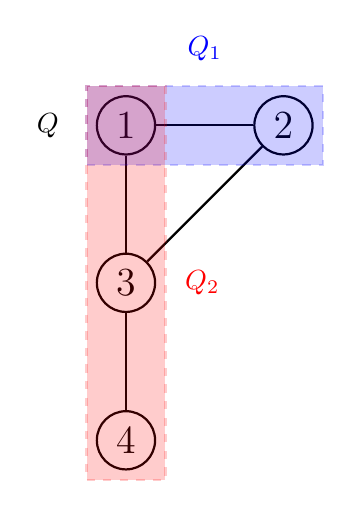
\begin{tikzpicture}[baseline=(current bounding box.north),-,auto,node distance=2cm,
                    thick,main node/.style={circle,draw,font=\sffamily\Large\bfseries}]

  \node[main node] (1) {$1$};
  \node[main node] (2) [right of=1] {$2$};
  \node[main node] (3) [below of=1] {$3$};
  \node[main node] (4) [below of=3] {$4$};

  \path[every node/.style={font=\sffamily}]
    (1) edge  (2)
    edge (3)
    (2) edge (3)
    (3) edge (4);
  
  \node (Box1) [draw=blue,dashed,thick,fit=(1) (2),fill=blue,opacity=0.2] {};  
  \node (Box2) [draw=red,dashed,thick,fit=(1) (3) (4),fill=red,opacity=0.2] {};
  
  \node [yshift=3.0ex, blue] at (Box1.north) {$Q_{1}$};
  \node [xshift=3.0ex, red] at (Box2.east) {$Q_{2}$};  
\node [left=0.5cm,text width=0.5cm] at (1)
{
$Q$
};   
\end{tikzpicture}
\end{center}
\caption{Decomposition of Q into \textcolor{blue}{$Q_{1}$} and \textcolor{red}{$Q_{2}$}.}
\label{examplefig:Q Decompisition}
\end{myfigure}

\textbf{Simplification(Patroller and Attacker):}

\begin{definition}[Node Identification]
The operation of Node identification on two nodes, $u$ and $v$, of a graph, $G=(N,E)$ into a single node $w$, is a mapping $f:N \rightarrow N'$ resulting in a new graph $G'=(N',E')$ where $N'=(N \setminus  \{u,v\}) \cup \{w\}$ with $E'=E \setminus \{(u,v)\}$ if $(u,v) \in E$ and under the condition that $\forall x \in N$, $f(x) \in N'$ is incident to $e' \in E'$ iff $e \in E$ is incident to $x \in N$.
Furthermore if a graph, $Q$, undergoes repeated node identification to become $Q'$ then we say it has been simplified. 
\end{definition}

\begin{definition}[Embedded walk]
An \textit{Embedded walk}, $W'$, on $Q'$ is the walk, $W$, done on $Q$ under the simplification mapping of $Q$ to $Q'$. i.e if $\pi :Q \rightarrow Q'$ is the simplification map, then $W'=\pi (W)$.
\end{definition}

\begin{lemma}[Simplification]
If $Q'$ is a simplified version of $Q$ then $V(Q') \geq V(Q)$
\end{lemma}

This allows us to get bounds for both the patroller and attacker.

\begin{example}
For $Q$ as seen in Figure \ref{fig: Q}. Consider when $m=3$, the Simplification of the graph by identifying $1,2$ from $Q$ to $Q'=L_{3}$ (as seen in Example Figure \ref{examplefig:Q Simplification}). Hence we can get the bound that $V(L_{3}) \geq  V(Q)$ hence $V(Q) \leq \frac{3}{4} $
\end{example}

\begin{myfigure}
\begin{center}
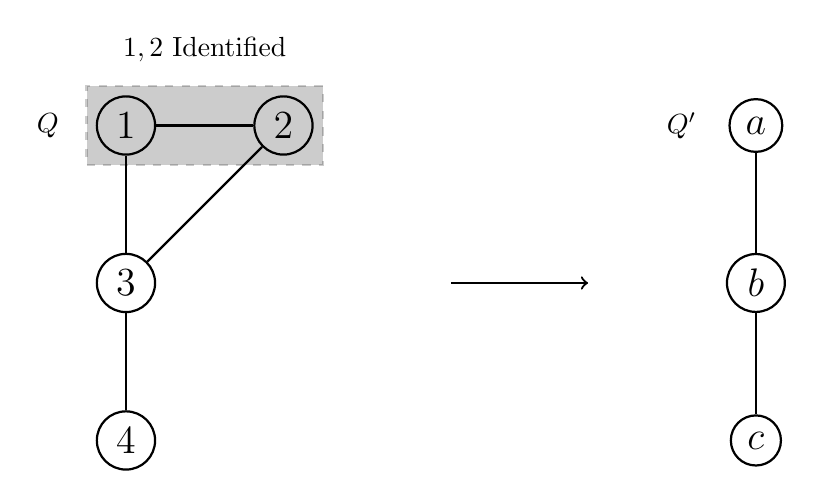
\begin{tikzpicture}[baseline=(current bounding box.north),-,auto,node distance=2cm,
                    thick,main node/.style={circle,draw,font=\sffamily\Large\bfseries}]

  \node[main node] (1) {$1$};
  \node[main node] (2) [right of=1] {$2$};
  \node[main node] (3) [below of=1] {$3$};
  \node[main node] (4) [below of=3] {$4$};
  
  \node (P1) [below of=2] {};
  \node (P2) [right of=P1] {};
  \node (P3) [right of=P2] {};
  
  \draw[->] (P2) edge (P3);
  
  \node[main node] (b) [right of=P3] {$b$};
  \node[main node] (a) [above of=b] {$a$};
  \node[main node] (c) [below of=b] {$c$};

  \path[every node/.style={font=\sffamily}]
    (1) edge  (2)
    edge (3)
    (2) edge (3)
    (3) edge (4)
    (a) edge (b)
    (b) edge (c);
  
  \node (Box1) [draw,dashed,thick,fit=(1) (2),fill,opacity=0.2] {};  
  
  \node [yshift=3.0ex] at (Box1.north) {$1,2$ Identified};  
\node [left=0.5cm,text width=0.5cm] at (1) {$Q$};
\node [left=0.5cm,text width=0.5cm] at (a) {$Q'$};   
\end{tikzpicture}
\end{center}
\caption{Simplifcation of $Q$ to $Q'$ by identification.}
\label{examplefig:Q Simplification}
\end{myfigure}


\textbf{Diametric attack(Attacker)}

Let $d(i,i')$ is the distance between nodes $i$ and $i'$ with the distance measured by the minimum number of edges.

\begin{definition}[Graph Diameter]
The diameter of a graph $Q$ is definded by $\bar{d}=\max\limits_{i,i' \in N} d(i,i')$ . The node pairs satisfying this are called diametrical.
\end{definition}

\begin{lemma}
By the attacker playing equally likely at a pair of diametrical at a random time interval, called the diametric attack, gives $V \leq \max\left\{\frac{m}{\raisebox{-0.5ex}{$\scriptstyle 2 \bar{d}$}} , \frac{1}{2} \right\}$
\end{lemma}

However the bound presented in \citep{Alpern2011} seems to indicate for large $T,m$ the second is chosen. However a simple counter example will show the bound does not allows hold
\begin{example}[Problem with diametric attack]
\label{example:counterexamplediamater} 
Consider the graph $L_{5}$ so $\bar{d}=4$ for $T=m=5$, then under the diametric attack, the patroller performing the patrol $\{ 1,2,3,4,5 \}$ allows her to catch the two attacks. Hence the bound of $V \leq \frac{5}{8}$ given by lemma does not seem to hold. 
\end{example}



\textbf{Covering(Patroller) and Independence(Attacker):}

\begin{definition}[Covering]
A patrol, $W$, is called \textit{intercepting} if it intercepts every possible attack at every node contained in the patrol, i.e all nodes visited by $W$ are in any subpath of length $m$ (i.e visits are at most $m$ apart).

A set of intercepting patrols forms a \textit{Covering set} if every node in $Q$ is contained in at least one of the patrols. Furthermore the \textit{Covering number}, $\mathcal{C}$ is the minimum cardinality of all the covering sets.
\end{definition}

\begin{definition}[Independence]
Two nodes, $i$ and $i'$, are called independent (under attack time, $m$) if any patrol intercepting an attack at $i$ cannot also intercept an attack at $i'$.

For the one-off game this is equivalent to $d(i,i') \geq m$.

For the Periodic game this is equivalent to $d(i,i') \geq m$ and $2d(i,i') \leq T$(due to returning to start).

A set of independent points forms a \textit{Independent set} if every element of the set is independent of every other element. Furthermore the independence number $\mathcal{I}$ is the maximum cardinality of all the independent sets.
\end{definition}

Clearly $\mathcal{I} \leq \mathcal{C}$ as to cover a collection of independent nodes, at least that many covering patrols are needed (Possibly more if they also don't get every node in $Q$)

\begin{lemma}[Covering and Independence]
$$ \frac{1}{\mathcal{C}} \leq V \leq \frac{1}{\mathcal{I}} $$
\end{lemma}

\subsubsection{Solved Graphs}
We shall provide some information on graphs that have already been solved

\textbf{Hamiltonian:}

A Hamiltonian graph is a graph with a Hamiltonian cycle(See Appendix [Blank] for a formal definition). Two simple examples of such graphs are cyclic graphs, $C_{n}$ and the complete graph, $K_{n}$. While Hamiltonian graphs can exhibit more than one Hamiltonian cycle we shall assume that we have selected one. We shall also assume that the attack, $m < n$, as otherwise by following the Hamiltonian cycle we guarantee capture (i.e for $m \geq n \implies V=1$).

\begin{definition}[Random Hamiltonian Patrol]
A \textit{Random Hamiltonian Patrol} is a mixed strategy starting with equal probability at all nodes and following the Hamiltonian cycle.
\end{definition}

\begin{theorem}[Hamiltonian]
If $Q$ is Hamiltonian, by following the Random Hamiltonian Patrol (if feasible), the patroller can achieve $V \geq \frac{m}{n}$.
\end{theorem}

This, along with a general upper bound from \citep{Alpern2011}, provides the solution $V=\frac{m}{n}$.

\textbf{Line:}

A Line Graph, $L_{n}$, is a graph consisting of $n$ nodes and $n-1$ edges connected in a straight line.  While the line graph is complicated it has been solved across; Patrolling Games \cite{Alpern2011} and Patrolling a Border \cite{Papadaki2016}. The cases in the solution require the division of the $(n,m)$ space into sub-regions (inside which different strategies are adopted by the attacker and patroller).

However upon investigation one of the sub-regions and strategies does not produce the correct bound as reported. We bring this up as in section \ref{Subsection:Problem and correction to line graph strategy} we will provide a counter-example to show the error and provide an altered strategy giving the required bound.

\textbf{Bipartite:}

A bipartite graph is a graph which can be partitioned into two sets, $A$ and $B$ (with $|A|=a,|B|=b$, assume WLOG that $b \geq a$) were edges only exist between these two sets. A special bipartite graph is the complete bipartite graph $K_{a,b}$.

Assume that $m < 2b$, as otherwise there exists a $2b$ period patrol which covers all nodes and guarantees capture (i.e if $m \geq 2b  \implies V=1$).

\begin{definition}[Bipartite Attack]
The \textit{Bipartite Attack} selects nodes equiprobably from the larger set $B$ for a fixed time interval, $I$ (or for the two time intervals, $I$ and $I+1$ equiprobably).
\end{definition}

\begin{theorem}[Bipartite]
If $Q$ is bipartite with $b \geq a$, by following the Bipartite Attack, the attacker can achieve $V \leq \frac{m}{2b}$
\end{theorem}

The reasoning behind the bound is that any patrol must alternate between $|A|$ and $|B|$, so only visits a node from $B$ every other time step. 

\begin{corollary}[Complete Bipartite]
\label{Corollary:Complete Bipartite}
The value of the complete bipartite graph, $K_{a,b}$, with $b \geq a$, then $V=\frac{m}{2b}$
\end{corollary}

This is because a lower bound of $V \geq \frac{m}{2b}$ is given by the random Hamiltonian patrol in $K_{b,b}$ , which simplifies to $K_{a,b}$.

\subsection{Patrolling games with random attackers}
\label{Section:Patrolling games with random attackers}
This section summarizes the key work from \cite{Lin2013} and their work on Patrolling games with random attackers. Providing a baseline for future work done in Section \ref{Section:Patrolling games with random attackers and local-observations}

\subsubsection{Game Set-up}
A patrolling game is random attackers, $G=G(Q,\bm{X},\bm{\lambda},\bm{c})$ is a minimizing game for the patroller. The parameters of the game are

\begin{itemize}
\item The graph $Q=(N,E)$ made of nodes, $N$ ($|N|=n$), joined by edges, $E$, which can be represented by an adjacency matrix, $A$.
\item A vector of attack time distributions, $\bm{X}=(X_{1},...,X_{n})$.
\item A vector of poisson arrival rates, $\bm{\lambda}=(\lambda_{1},...,\lambda_{n})$.
\item A vector of costs, $\bm{c}=(c_{1},...,c_{n})$
\end{itemize}

\begin{myfigure}
\begin{center}
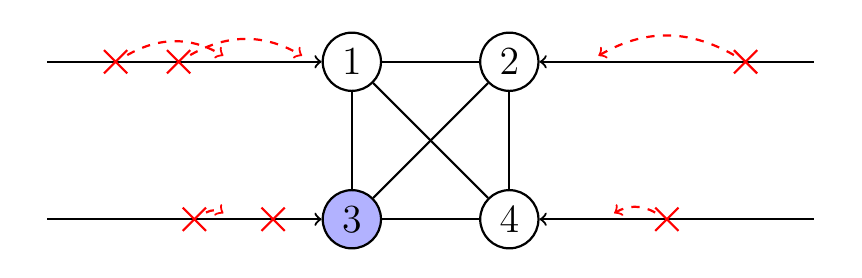
\begin{tikzpicture}[-,auto,node distance=2cm,
                    thick,main node/.style={circle,fill=white,draw,font=\sffamily\Large\bfseries}]

%DRAWING GRAPH
  \node[main node] (1) {$1$};
  \node[main node] (2) [right of=1] {$2$};
  \node[main node,fill=blue!30] (3) [below of=1]  {$3$};
  \node[main node] (4) [below of=2]  {$4$};

  \path[every node/.style={font=\sffamily}]
    (1) edge (2)
        edge (3)
        edge (4)
    (2) edge (3)
        edge (4)
    (3) edge (4);
  
  
%DRAWING ARRIVALS  
  \node (1ArrowStart) [shift={(-4,0)}] at (1) {};
  \draw[->] (1ArrowStart)--(1);
  
  \node[cross=5pt,color=red] (1Cross1) [shift={(-3,0)}] at (1) { };
  \node (1CrossEnd1) [shift={(-1.5,0)}] at (1) {};
  \draw[->,bend left,dashed,color=red] (1Cross1) to (1CrossEnd1);
  \node[cross=5pt,color=red] (1Cross2) [shift={(-2.2,0)}] at (1) { };
  \node (1CrossEnd2) [shift={(-0.5,0)}] at (1) {};
  \draw[->,bend left,dashed,color=red] (1Cross2) to (1CrossEnd2);
  
  \node (2ArrowStart) [shift={(4,0)}] at (2) {};
  \draw[->] (2ArrowStart)--(2);
  
  \node[cross=5pt,color=red] (2Cross1) [shift={(3,0)}] at (2) { };
  \node (2CrossEnd1) [shift={(1,0)}] at (2) {};
  \draw[->,bend right,dashed,color=red] (2Cross1) to (2CrossEnd1);

  \node (3ArrowStart) [shift={(-4,0)}] at (3) {};
  \draw[->] (3ArrowStart)--(3);
  
  \node[cross=5pt,color=red] (3Cross1) [shift={(-2,0)}] at (3) { };
  \node (3CrossEnd1) [shift={(-1.5,0)}] at (3) {};
  \draw[->,bend left,dashed,color=red] (3Cross1) to (3CrossEnd1);
  \node[cross=5pt,color=red] (3Cross1) [shift={(-1,0)}] at (3) { };
  
  \node (4ArrowStart) [shift={(4,0)}] at (4) {};
  \draw[->] (4ArrowStart)--(4);
  
  \node[cross=5pt,color=red] (4Cross1) [shift={(2,0)}] at (4) { };
  \node (4CrossEnd1) [shift={(1.2,0)}] at (4) {};
  \draw[->,bend right,dashed,color=red] (4Cross1) to (4CrossEnd1);
    
\end{tikzpicture}
\end{center}
\caption{Example of $G=(K_{4},\bm{X},\bm{\lambda},\bm{c})$ with patroller currently at node $3$}
\end{myfigure}

The attackers arrive at node, $i$, according a poisson process of rate $\lambda_{i}$, beginning their attack immediately, which lasts $X_{i}$ time. The patroller detects all ongoing attacks when arriving at node $i$, the patroller then moves taking unit time to arrive at the next node (which can be the current node).

\begin{myfigure}
\begin{center}
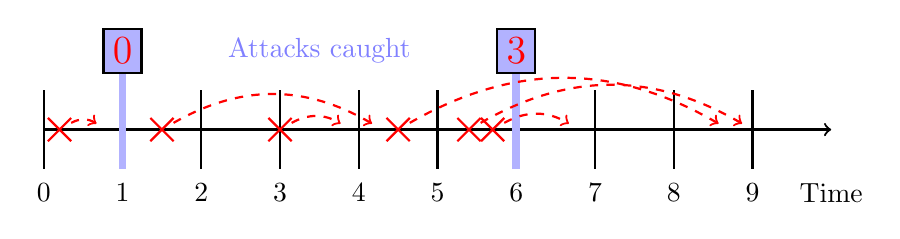
\begin{tikzpicture}[-,auto,node distance=2cm,
                    thick,main node/.style={rectangle,draw,font=\sffamily\Large\bfseries}]

%DRAWING Base line

 \draw[->] (0,0)--(10,0);
 
 \foreach \x in {0,...,9}
 {\draw  (\x,0.5)--(\x,-0.5) ;
  \node (TimeLabel\x) at (\x,-0.8) {$\x$};} 
  
  \node (TimeLabel) at (10,-0.8) {Time};

%Inserting patroller and attackers
  \node[main node,fill=blue!30] (Pat1) at (1,1) {\textcolor{red}{$0$}};
  \draw[color=blue!30,line width=0.1cm] (Pat1)--(1,-0.5);
  
  \node[main node,fill=blue!30] (Pat2) at (6,1) {\textcolor{red}{$3$}};
  \draw[color=blue!30,line width=0.1cm] (Pat2)--(6,-0.5);
  
  \node[cross=5pt,color=red] (AttackStart1) at (0.2,0) {};
  \node (AttackEnd1) at (0.8,0) {};
  \draw[bend left,color=red,->,dashed] (AttackStart1) to (AttackEnd1);
  
  \node[cross=5pt,color=red] (AttackStart2) at (1.5,0) {};
  \node (AttackEnd2) at (4.3,0) {};
  \draw[bend left,color=red,->,dashed] (AttackStart2) to (AttackEnd2);
  
  \node[cross=5pt,color=red] (AttackStart3) at (3,0) {};
  \node (AttackEnd3) at (3.9,0) {};
  \draw[bend left,color=red,->,dashed] (AttackStart3) to (AttackEnd3);
  
  \node[cross=5pt,color=red] (AttackStart4) at (4.5,0) {};
  \node (AttackEnd4) at (8.7,0) {};
  \draw[bend left,color=red,->,dashed] (AttackStart4) to (AttackEnd4);
  
  \node[cross=5pt,color=red] (AttackStart5) at (5.4,0) {};
  \node (AttackEnd5) at (9,0) {};
  \draw[bend left,color=red,->,dashed] (AttackStart5) to (AttackEnd5);
  
  \node[cross=5pt,color=red] (AttackStart6) at (5.7,0) {};
  \node (AttackEnd6) at (6.8,0) {};
  \draw[bend left,color=red,->,dashed] (AttackStart6) to (AttackEnd6);
  
  
  \node (AttacksCaught) at (3.5,1) {\textcolor{blue!50}{Attacks caught}};
       
\end{tikzpicture}
\end{center}
\caption{Example for a given node, when the patroller visits at times, $1,5$}
\end{myfigure}

We can formulate such as problem as a Markov Decision Process(MDP) with state space, $\Omega= \{\bm{s}=(s_{1},...,s_{n}) \, | \, s_{i}=1,2,... \, \text{ for } i=1,...,n \}$,  where $s_{i}$ denotes the time period since the decision to last visit node $i$ was taken. Because the patroller can only visit one node per time period, all $s_{i}$ have distinct values. In particular, one $s_{i}$, the current node, has value $1$. We can identify the current node by $l(\bm{s})=\argmin_{i} s_{i}$. The available decisions from state $\bm{s}$ are $\mathcal{A}(\bm{s})=\{j | A_{l(\bm{s}),j}=1 \}$ and when node $i$ is chosen by the patroller the state transitions to $\phi(\bm{s},i)=\widetilde{\bm{s}}$, where $\widetilde{s}_{i}=1$ and $\widetilde{s}_{j}=s_{j}+1 \; \forall j \neq i$.

Because the future of the process is independent of its past, it is only the current state that matters, we can formulate its movement as a Markov Chain(MC) and hence the patroller's problem is a MDP.

The patroller incurs costs for all attackers able to complete their attacks. For the decision the cost in the next time period is the sum of all costs incurred at all nodes, I.e $C(\bm{s},i)=\sum\limits_{j=1}^{j=n} C_{j}(\bm{s},i)$ , where $C_{j}(\bm{s},i)$ is the cost at node $j$ choosing to move to node $i$ in the next time period. Hence

\begin{align*}
C_{j}(\bm{s},i)&=c_{j} \lambda_{j} \int_{0}^{s_{j}} P(t-1 < X_{j} \leq t) dt \\
&=c_{j} \lambda_{j} \int_{s_{j}-1}^{s_{j}} P(X_{j} \leq t) dt
\end{align*}

\begin{note}
$C_{j}(\bm{s},i)$ is not dependent on $i$, the choice of $i$ affects the future state (and hence future incurred costs)
\end{note}
  
With a countable infinite state space, $\Omega$, problems of finding an optimal policy may exisit (See [Need reference from Peuterman]), so we bound the state space to make it finite. A reasonable assumption is to bound the attack times and define, the smallest interger for this bound

\begin{align}
\label{Equation:Definition of attack time bound}
B_{j} \equiv \min \{ k \, | \, k \in \mathbb{Z}^{+} , P(X_{j} \leq k)=1 \}
\end{align}

We now see that the cost function remains constant, $c_{j} \lambda_{j}$, for all $s_{j} \geq B_{j}+1$ and so we restrict our state space to $s_{j} \leq B_{j}+1$ and modify the transitions slightly so $\widetilde{s}_{j}=\min(s_{j}+1,B_{j}+1) \; \forall j \neq i$.

Now we can consider the objective function for our MDP, we wish to minimize the long-run average cost incurred. We also know by [reference to peuterman], that we can just focus on the class of stationary, deterministic policies $\Pi= \{\pi: \Omega \rightarrow N \, |\,\pi(\bm{s}) \in \mathcal{A}(\bm{s}) \}$. So we wish to solve

\begin{align*}
C^{\text{OPT}}(\bm{s}_{0}) \equiv \min\limits_{\pi \in \Pi} \sum\limits_{i=1}^{n} V_{i}(\pi,\bm{s}_{0})
\end{align*}

Where $V_{i}(\pi,\bm{s}_{0})$ is the long-run average cost incurred at node $i$ under the policy, $\pi$, starting from state, $(\bm{s}_{0})$ defined by ,

\begin{align*}
V_{i}(\pi,\bm{s}_{0}) \equiv \lim\limits_{N \rightarrow \infty} \frac{1}{N} \sum\limits_{k=0}^{N-1} C_{i}(\phi^{k}_{\pi}(\bm{s}_{0}),\pi(\phi^{k}_{\pi}(\bm{s}_{0})))
\end{align*}
Where $\phi^{k}_{\pi}(\bm{s}_{0})$ is the state after $k$ transitions starting from $(\bm{s}_{0})$ under the policy $\pi$.

Because the transitions are deterministic and the state space is finite, we know that $\phi^{k}_{\pi}(\bm{s}_{0})$ will repeat and induce a cyclic behaviour under the policy,$\pi$. We will define the patrol pattern to be exactly this, from $\bm{s}_{0}$ let $\bm{s}_{R}$ be the first state which is repeated then define $\psi^{k}_{\pi}=\phi^{k}_{\pi}(\bm{s}_{R})$, so the patrol pattern is $\{\psi^{k}_{\pi} \, | \, k=0,1,...,K-1 \}$. We say the patrol pattern is of length $K$. We can rewrite the long-run average cost at a node to be

\begin{align*}
V_{i}(\pi,\bm{s}_{0})=\frac{1}{K} \sum\limits_{k=0}^{K-1} C_{i}(\psi^{k}_{\pi},\pi(\psi^{k}_{\pi}))
\end{align*}

We will assume we are dealing with a connected graph, otherwise we solved the connected parts separately. Therefore, because every state is reachable we see that $C^{\text{OPT}}(\bm{s}_{0})$ does not depend on the initial state and so $C^{\text{OPT}}=C^{\text{OPT}}(\bm{s}_{0})$ is the same for all initial states.

\begin{note}
If we set $c_{i}=1 \; \forall i$ then we can interest the long-run average cost, as the probability of not detecting an attack.
\end{note}

We can now use standard techniques such as value iteration or linear programming to compute the optimal policy and long-run average cost. This is left to Appendix \ref{Appendix:Optimal Solution for a Random Attacker}. However such methods are slow are only computable for a small graph, therefore we seek to create a near-optimal heuristic policy that can run in a shorter space of time.


\subsubsection{Problem relaxation}
We first relax the problem of the patroller only being able to visit one adjacent node each time period, to the \textit{Multi-Node}(MN) problem, where the patroller can visit multiple nodes each time period. We will denote the class of stationary, deterministic policies as

\begin{align*}
\Pi^{\text{MN}}=\{\pi^{n}: \Omega \rightarrow \bm{\alpha} \, | \alpha_{i}=0,1 \text{ for } i=1,...,n \}
\end{align*}

For ease of notation we will define $\pi_{i}:\Omega \rightarrow \alpha_{i} \in \Pi^{\text{MN}}_{i}$, that is the resultant element map, which we will use when we only care about a single node.

\begin{note}
Our previous un-relaxed policies, $\pi: \Omega \rightarrow N$ can be converted to a MN policy by mapping $\bm{s}$ to $\bm{\alpha}$ where $\alpha_{i}=1$ for $i=\pi(\bm{s})$ and $\alpha_{i}=0$ for $i \neq \pi(\bm{s})$ to form a policy $\pi^{n} \equiv \pi$.
\end{note}

Like before $\pi^{n}$ will induce a patrol pattern, $\psi^{k}_{\pi^{n}}$ with length $K'$. We define the long-run average visit rate at which node, $i$ is visited to be under $\pi^{n}$ starting from $\bm{s}_{0}$ as

\begin{align*}
\mu_{i}(\pi_{i},\bm{s}_{0})=\frac{1}{K'} \sum\limits_{k=0}^{K'-1} \pi_{i}(\psi^{k}_{\pi^{n}})
\end{align*}

Now we restrict ourselves to having a maximum long-run average visit rate of one. This is know as the \textit{Total-Rate}(TR) constraint. So we restrict ourselves to obey this constraint and the set of policies,

\begin{align*}
\Pi^{\text{TR}}=\left\{ \pi^{n} \in \Pi^{\text{MN}} \, \bigg| \, \sum\limits_{i=1}^{N} \mu_{i}(\pi_{i},\bm{s}_{0}) \leq 1 \, , \, \forall \bm{s}_{0} \in \Omega \right\}
\end{align*}

We define the Problems optimal minimum cost, $C^{\text{TR}}=\min\limits_{\pi^{n} \in \Pi^{\text{TR}}} \sum\limits_{i=1}^{n} V_{i}(\pi^{n})$, similarly to before.

\begin{note}
We have dropped the dependency on the initial state, $\bm{s}_{0}$, as even though $V_{i}(\pi^{n},\bm{s}_{0})$ depends on it, the long-run average cost does not. We will similarly drop the notation on the long-run visit rate, using $\mu_{i}(\pi^{n})$.
\end{note}

Again,  $\exists \; \pi^{n} \in \Pi^{\text{TR}} \text{ s.t } \pi \equiv \pi^{n}$, so $C^{\text{OPT}} \geq C^{\text{TR}} $

Secondly we relax the MN problem by introducing the TR constraint as a Lagrangian multiplier, $\omega \geq 0$, to form

\begin{align*}
C(\omega) & \equiv \min\limits_{\pi^{n} \in \Pi^{\text{MN}}} \left(\sum\limits_{i=1}^{n} V_{i}(\pi^{n}) + \omega \left(\sum\limits_{i=1}^{n} \mu_{i}(\pi^{n}) -1\right) \right) \\
&= \min\limits_{\pi^{n} \in \Pi^{\text{MN}}} \sum\limits_{i=1}^{n} \left(V_{i}(\pi^{n}) + \omega \mu_{i}(\pi^{n})\right)  -\omega
\end{align*}

This formulation means that $C^{\text{TR}} \geq C(\omega)$, hence $C^{\text{OPT}} \geq C^{\text{TR}} \geq C(\omega)$.

The Lagrangian relaxtion can be interpreted as the cost of missed attacks plus a cost of $\omega$ for ever visit we make, therefore we call $\omega$ the \textit{service charge}. As the Lagrangian relaxation, splits up into $n$ separate problems, where node $i$'s problem is

\begin{align*}
C_{i}(\omega) \equiv \min\limits_{\pi_{i} \in \Pi^{\text{MN}}_{i}} \left(V_{i}(\pi_{i}) + \omega \mu_{i}(\pi_{i})\right)
\end{align*}

With $C(\omega)=\left(\sum\limits_{i}^{n} C_{i}(\omega)\right) -\omega$

\subsubsection{Single-node problem}

Focusing on the separated, single node problem is equivalent to deciding when to visit the node. We shall remove node subscript, $i$, for ease of reading. Each time has a binary decision, visit ($1$) or wait ($0$). Because we are only considering stationary, deterministic policies, the optimal action of when to visit remains constant and the optimal policy will be one that visits every, $k$ periods. Such a policy gives us an expected number of arrivals who finish before we visit of

\begin{align*}
\lambda \int_{0}^{k} P(X \leq k-t) dt= \lambda \int_{0}^{k} P(X \leq t) dt
\end{align*}

Each successful attack costs $c$ and the visit costs us $\omega$ and this cycle is of length $k$ so the long-run average cost is

\begin{align*}
f(k) \equiv \frac{c \lambda \int_{0}^{k} P(X \leq t) dt + \omega}{k}
\end{align*}

Thus solving the single node problem is equivalent to minimizing $f(k)$, by setting $f(k) = f(k+1)$ we can find the cost that makes the patroller indifferent between visiting every $k$ and $k+1$ time units. This solution helps us characterise the optimal policy that minimizes $f(k)$ defined as

\begin{align*}
W(k) \equiv c \lambda \left( k \int_{k}^{k+1} P(x \leq t) dt - \int_{0}^{k} P(x \leq t) dt \right)
\end{align*}

We have $W(0)=0$ and as $X$ is bounded by $B$, we have for $k \geq B$ that $W(k)= c \lambda E[X]$. We us this function to characterise the optimal policy minimizing the single node objective

\begin{theorem}[Single node optimal policy]
\label{Theorem:Single node optimal policy}
\begin{itemize}
\item[a)] $W(k)$ is non-decreasing in $k$.
\item[b)] If $\omega \in [W(k-1),W(k)]$ then it optimal to visit the node once every $k$ time periods, for $k=1,2,...$
\item[c)] Moreover if $\omega \geq c \lambda E[X]$ it is never optimal to visit the node.
\end{itemize}
\end{theorem}

Proof: See Appendix \ref{Appendix:Optimal Solution for a Random Attacker}

This motivates a simple Index Heuristic(IH) based on the optimal solution to the single node problem, by reinserting the node subscript, we suggest an index of

\begin{align*}
W_{i}(\bm{s}) \equiv c_{i} \lambda_{i} \left(s_{i} \int_{s_{i}}^{s_{i}+1} P(X_{i} \leq t) dt - \int_{0}^{s_{i}} P(X_{i} \leq t) dt \right)
\end{align*}

The IH computes the index for all adjacent nodes (including the current node) from the state $\bm{s}$ and moves to the node with the highest index. In the cases of ties in indices, they are broke arbitrarily.

\subsubsection{More heuristics}
The IH is simplistic and short sighted, we can develop more sophisticated heuristics based on the index.

\textbf{Index Reward Heuristic(IRH)}
We can interpret the index as a reward for visiting the node and pick a look-ahead window of length $l$, we then look at all paths of length $l$ from the current node, aggregating the index along the path. Then choosing the next node to visit according to which path has the highest aggregate reward.

\textbf{Index Penalty Heuristic(IPH)}
We could also interpret the index as a penalty for not visiting the node. With a look-ahead window of length $l$, we look at all paths of length $l$ from the current node, aggregating the indices not along the path. Then choosing the next node to visit according to which path has the lowest aggregate penalty. 

\begin{note}
We only use the aggregate reward/penalty to determine the next node, then we repeat the process, we do not follow the path.
\end{note}

A natural question to ask is; does increasing the look-ahead window improve the heuristic. The answer is no, as $l$ and $l+1$ may return two distinct patrol patterns, with $l$'s patrol pattern performing better than $l+1$'s. However when considering using a look-ahead window of $l+1$ we have to compute $l$'s paths, so we might as well look at all look-ahead windows up to a value. We shall call this the heuristic depth, $d$ and denote the depth heuristics as IRH($d$) and IPH($d$) which apply IRH and IPH respectively to all look-ahead windows of length $l=1,...,d$.

\begin{note}
IRH($1$) $\equiv$ IPH($1$)
\end{note}

The numerical results of these heuristics can be found in Section 3.4 in \citep{Lin2013}. A key result of the study, that we will look at later is that IPH seems to outform IRH on the Complete and Line graph.

\section{Strategic Patroller and Strategic Attacker}

\subsection{Problem and correction to line graph strategy}
\label{Subsection:Problem and correction to line graph strategy}
Consider the patroller's strategy against a diametric attack, that simply oscillates between the two diametric points.

The total number of attacks the attacker is making under this diametric strategy is $2(T-m+1)$, we will now measure how many the simple strategy for the patroller gets.

We will divide the set of captured attacks, depending on what is happening. This division shall be into start captures, middle captures and end captures.

The start captures are captures catching less than $m$ attacks in the early times, i.e before the middle. The middle captures are captures catching exactly $m$ attacks. The end captures are captures catching less than $m$ attacks in the late times.

\begin{example}[Problem with diametric attack]
Consider the graph $L_{5}$ so $\bar{d}=4$ for $T=20$,$m=6$, then under the diametric attack, the patroller oscillating between diametrics points gets.
\begin{itemize}
\item[Start] Capture $1+5=6$ attacks initially.
\item[Middle] Capture $6+6=12$ attacks when arriving at node $5$.
\item[End] Capture $4$ attacks when finishing at node $1$.
\end{itemize}
Giving $22$ out of $2(20-6+1)=30$ attacks, a better than $\frac{3}{4}$ value.
\end{example}

First off it is worth considering that the number of end attacks that are going to be caught will come from two values (if more than these would be in the middle). We could suggest that waiting at the start is more preferable to ``stabilize'' into the middle quicker. the cost for doing so is to remove one from each end value, if one of the end values is 1, then the penultimate middle is also reduced by 1 and thus becomes an end value.

While each time we decide to wait gains us 1 for each node in the start values, until it becomes a middle value. As $m \geq \bar{d}$, we are guaranteed that there are at least two start values (as we are looking at times $0$ and $\bar{d}-1 < m$). Therefore it is certain that waiting at the start (at least while there are two start values) is not worse than the just oscillating strategy.

Therefore we can wait until $t=m-(\bar{d}-1)$ (which as $m > \bar{d}-1$ means its is always possible), then this is only the start.

Let us count the pattern under this strategy,
\begin{itemize}
\item[Start:] Capture $m-\bar{d}$ attacks initially by waiting.
\item[Middle:] Capture $m \times (\floor{\frac{T-2m+1}{\bar{d}}}+1)$ attacks in the middle cycles (if any middle times are possible, otherwise zero if negative).
\item[End:] Capture $T-1-(m-1+(\floor{\frac{T-2m+1}{\bar{d}}}+1)\bar{d})$ (at the penultimate node visit (if possible, this really is zero if its negative) and $T-1-(m-1+(\floor{\frac{T-2m+1}{\bar{d}}}+2)\bar{d})$ at the final node visit (again zero if negative).
\end{itemize}

This gives \begin{align*}
& m-\bar{d}+\pospart{m \times (\floor{\frac{T-2m+1}{\bar{d}}}+1)} + \\ &\pospart{T-(m-1+(\floor{\frac{T-2m+1}{\bar{d}}}+1)\bar{d})} + \pospart{T-(m-1+(\floor{\frac{T-2m+1}{\bar{d}}}+2)\bar{d})}
\end{align*}

We will call $\alpha=\floor{\frac{T-2m+1}{\bar{d}}}$

\begin{lemma}[Condition on $T$ for bound to hold]
When $T=m-1+(k+1)\bar{d}$ for some $k \in \mathbb{N}_{0}$ then the diametric bound holds. Otherwise as $T \rightarrow \infty$ then the diametric bound holds.
\end{lemma}

Proof: \ref{Condition on T for old diametric proof}

\begin{figure}
%\includegraphics[scale=0.4]{DiametricAttack(m_45,d_30)1.png}
\resizebox{0.95\linewidth}{!}{
% Created by tikzDevice version 0.10.1 on 2017-11-09 12:03:49
% !TEX encoding = UTF-8 Unicode
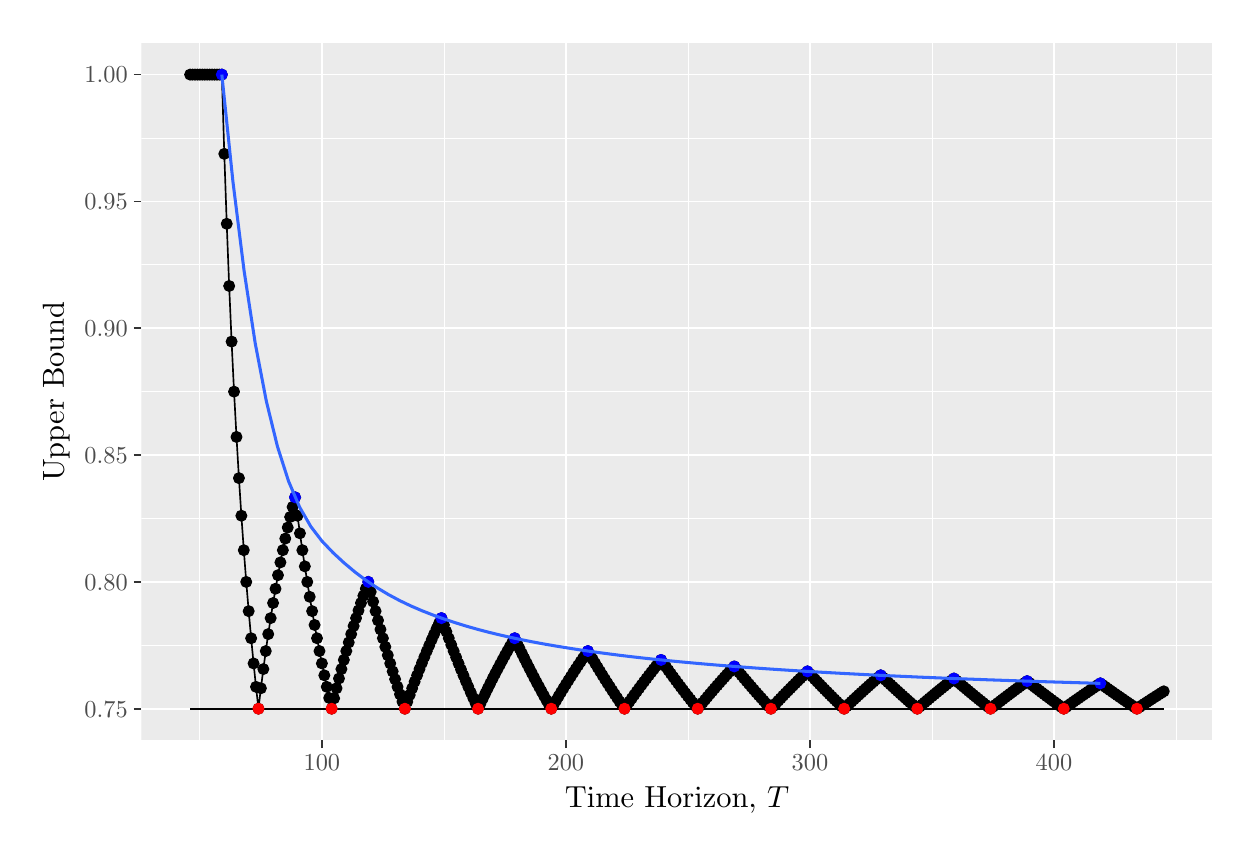
\begin{tikzpicture}[x=1pt,y=1pt]
\definecolor{fillColor}{RGB}{255,255,255}
\path[use as bounding box,fill=fillColor,fill opacity=0.00] (0,0) rectangle (433.62,289.08);
\begin{scope}
\path[clip] (  0.00,  0.00) rectangle (433.62,289.08);
\definecolor{drawColor}{RGB}{255,255,255}
\definecolor{fillColor}{RGB}{255,255,255}

\path[draw=drawColor,line width= 0.6pt,line join=round,line cap=round,fill=fillColor] (  0.00,  0.00) rectangle (433.62,289.08);
\end{scope}
\begin{scope}
\path[clip] ( 41.11, 31.53) rectangle (428.12,283.58);
\definecolor{fillColor}{gray}{0.92}

\path[fill=fillColor] ( 41.11, 31.53) rectangle (428.12,283.58);
\definecolor{drawColor}{RGB}{255,255,255}

\path[draw=drawColor,line width= 0.3pt,line join=round] ( 41.11, 65.90) --
	(428.12, 65.90);

\path[draw=drawColor,line width= 0.3pt,line join=round] ( 41.11,111.73) --
	(428.12,111.73);

\path[draw=drawColor,line width= 0.3pt,line join=round] ( 41.11,157.56) --
	(428.12,157.56);

\path[draw=drawColor,line width= 0.3pt,line join=round] ( 41.11,203.38) --
	(428.12,203.38);

\path[draw=drawColor,line width= 0.3pt,line join=round] ( 41.11,249.21) --
	(428.12,249.21);

\path[draw=drawColor,line width= 0.3pt,line join=round] ( 62.23, 31.53) --
	( 62.23,283.58);

\path[draw=drawColor,line width= 0.3pt,line join=round] (150.41, 31.53) --
	(150.41,283.58);

\path[draw=drawColor,line width= 0.3pt,line join=round] (238.58, 31.53) --
	(238.58,283.58);

\path[draw=drawColor,line width= 0.3pt,line join=round] (326.76, 31.53) --
	(326.76,283.58);

\path[draw=drawColor,line width= 0.3pt,line join=round] (414.94, 31.53) --
	(414.94,283.58);

\path[draw=drawColor,line width= 0.6pt,line join=round] ( 41.11, 42.99) --
	(428.12, 42.99);

\path[draw=drawColor,line width= 0.6pt,line join=round] ( 41.11, 88.81) --
	(428.12, 88.81);

\path[draw=drawColor,line width= 0.6pt,line join=round] ( 41.11,134.64) --
	(428.12,134.64);

\path[draw=drawColor,line width= 0.6pt,line join=round] ( 41.11,180.47) --
	(428.12,180.47);

\path[draw=drawColor,line width= 0.6pt,line join=round] ( 41.11,226.30) --
	(428.12,226.30);

\path[draw=drawColor,line width= 0.6pt,line join=round] ( 41.11,272.12) --
	(428.12,272.12);

\path[draw=drawColor,line width= 0.6pt,line join=round] (106.32, 31.53) --
	(106.32,283.58);

\path[draw=drawColor,line width= 0.6pt,line join=round] (194.49, 31.53) --
	(194.49,283.58);

\path[draw=drawColor,line width= 0.6pt,line join=round] (282.67, 31.53) --
	(282.67,283.58);

\path[draw=drawColor,line width= 0.6pt,line join=round] (370.85, 31.53) --
	(370.85,283.58);
\definecolor{drawColor}{RGB}{0,0,0}
\definecolor{fillColor}{RGB}{0,0,0}

\path[draw=drawColor,line width= 0.4pt,line join=round,line cap=round,fill=fillColor] ( 58.70,272.12) circle (  1.96);

\path[draw=drawColor,line width= 0.4pt,line join=round,line cap=round,fill=fillColor] ( 59.58,272.12) circle (  1.96);

\path[draw=drawColor,line width= 0.4pt,line join=round,line cap=round,fill=fillColor] ( 60.47,272.12) circle (  1.96);

\path[draw=drawColor,line width= 0.4pt,line join=round,line cap=round,fill=fillColor] ( 61.35,272.12) circle (  1.96);

\path[draw=drawColor,line width= 0.4pt,line join=round,line cap=round,fill=fillColor] ( 62.23,272.12) circle (  1.96);

\path[draw=drawColor,line width= 0.4pt,line join=round,line cap=round,fill=fillColor] ( 63.11,272.12) circle (  1.96);

\path[draw=drawColor,line width= 0.4pt,line join=round,line cap=round,fill=fillColor] ( 63.99,272.12) circle (  1.96);

\path[draw=drawColor,line width= 0.4pt,line join=round,line cap=round,fill=fillColor] ( 64.87,272.12) circle (  1.96);

\path[draw=drawColor,line width= 0.4pt,line join=round,line cap=round,fill=fillColor] ( 65.76,272.12) circle (  1.96);

\path[draw=drawColor,line width= 0.4pt,line join=round,line cap=round,fill=fillColor] ( 66.64,272.12) circle (  1.96);

\path[draw=drawColor,line width= 0.4pt,line join=round,line cap=round,fill=fillColor] ( 67.52,272.12) circle (  1.96);

\path[draw=drawColor,line width= 0.4pt,line join=round,line cap=round,fill=fillColor] ( 68.40,272.12) circle (  1.96);

\path[draw=drawColor,line width= 0.4pt,line join=round,line cap=round,fill=fillColor] ( 69.28,272.12) circle (  1.96);

\path[draw=drawColor,line width= 0.4pt,line join=round,line cap=round,fill=fillColor] ( 70.16,272.12) circle (  1.96);

\path[draw=drawColor,line width= 0.4pt,line join=round,line cap=round,fill=fillColor] ( 71.05,243.48) circle (  1.96);

\path[draw=drawColor,line width= 0.4pt,line join=round,line cap=round,fill=fillColor] ( 71.93,218.21) circle (  1.96);

\path[draw=drawColor,line width= 0.4pt,line join=round,line cap=round,fill=fillColor] ( 72.81,195.74) circle (  1.96);

\path[draw=drawColor,line width= 0.4pt,line join=round,line cap=round,fill=fillColor] ( 73.69,175.65) circle (  1.96);

\path[draw=drawColor,line width= 0.4pt,line join=round,line cap=round,fill=fillColor] ( 74.57,157.56) circle (  1.96);

\path[draw=drawColor,line width= 0.4pt,line join=round,line cap=round,fill=fillColor] ( 75.46,141.19) circle (  1.96);

\path[draw=drawColor,line width= 0.4pt,line join=round,line cap=round,fill=fillColor] ( 76.34,126.31) circle (  1.96);

\path[draw=drawColor,line width= 0.4pt,line join=round,line cap=round,fill=fillColor] ( 77.22,112.72) circle (  1.96);

\path[draw=drawColor,line width= 0.4pt,line join=round,line cap=round,fill=fillColor] ( 78.10,100.27) circle (  1.96);

\path[draw=drawColor,line width= 0.4pt,line join=round,line cap=round,fill=fillColor] ( 78.98, 88.81) circle (  1.96);

\path[draw=drawColor,line width= 0.4pt,line join=round,line cap=round,fill=fillColor] ( 79.86, 78.24) circle (  1.96);

\path[draw=drawColor,line width= 0.4pt,line join=round,line cap=round,fill=fillColor] ( 80.75, 68.45) circle (  1.96);

\path[draw=drawColor,line width= 0.4pt,line join=round,line cap=round,fill=fillColor] ( 81.63, 59.35) circle (  1.96);

\path[draw=drawColor,line width= 0.4pt,line join=round,line cap=round,fill=fillColor] ( 82.51, 50.89) circle (  1.96);

\path[draw=drawColor,line width= 0.4pt,line join=round,line cap=round,fill=fillColor] ( 83.39, 42.99) circle (  1.96);

\path[draw=drawColor,line width= 0.4pt,line join=round,line cap=round,fill=fillColor] ( 84.27, 50.38) circle (  1.96);

\path[draw=drawColor,line width= 0.4pt,line join=round,line cap=round,fill=fillColor] ( 85.16, 57.31) circle (  1.96);

\path[draw=drawColor,line width= 0.4pt,line join=round,line cap=round,fill=fillColor] ( 86.04, 63.82) circle (  1.96);

\path[draw=drawColor,line width= 0.4pt,line join=round,line cap=round,fill=fillColor] ( 86.92, 69.94) circle (  1.96);

\path[draw=drawColor,line width= 0.4pt,line join=round,line cap=round,fill=fillColor] ( 87.80, 75.72) circle (  1.96);

\path[draw=drawColor,line width= 0.4pt,line join=round,line cap=round,fill=fillColor] ( 88.68, 81.18) circle (  1.96);

\path[draw=drawColor,line width= 0.4pt,line join=round,line cap=round,fill=fillColor] ( 89.56, 86.34) circle (  1.96);

\path[draw=drawColor,line width= 0.4pt,line join=round,line cap=round,fill=fillColor] ( 90.45, 91.23) circle (  1.96);

\path[draw=drawColor,line width= 0.4pt,line join=round,line cap=round,fill=fillColor] ( 91.33, 95.86) circle (  1.96);

\path[draw=drawColor,line width= 0.4pt,line join=round,line cap=round,fill=fillColor] ( 92.21,100.27) circle (  1.96);

\path[draw=drawColor,line width= 0.4pt,line join=round,line cap=round,fill=fillColor] ( 93.09,104.46) circle (  1.96);

\path[draw=drawColor,line width= 0.4pt,line join=round,line cap=round,fill=fillColor] ( 93.97,108.45) circle (  1.96);

\path[draw=drawColor,line width= 0.4pt,line join=round,line cap=round,fill=fillColor] ( 94.85,112.26) circle (  1.96);

\path[draw=drawColor,line width= 0.4pt,line join=round,line cap=round,fill=fillColor] ( 95.74,115.89) circle (  1.96);

\path[draw=drawColor,line width= 0.4pt,line join=round,line cap=round,fill=fillColor] ( 96.62,119.37) circle (  1.96);

\path[draw=drawColor,line width= 0.4pt,line join=round,line cap=round,fill=fillColor] ( 97.50,112.72) circle (  1.96);

\path[draw=drawColor,line width= 0.4pt,line join=round,line cap=round,fill=fillColor] ( 98.38,106.37) circle (  1.96);

\path[draw=drawColor,line width= 0.4pt,line join=round,line cap=round,fill=fillColor] ( 99.26,100.27) circle (  1.96);

\path[draw=drawColor,line width= 0.4pt,line join=round,line cap=round,fill=fillColor] (100.15, 94.43) circle (  1.96);

\path[draw=drawColor,line width= 0.4pt,line join=round,line cap=round,fill=fillColor] (101.03, 88.81) circle (  1.96);

\path[draw=drawColor,line width= 0.4pt,line join=round,line cap=round,fill=fillColor] (101.91, 83.42) circle (  1.96);

\path[draw=drawColor,line width= 0.4pt,line join=round,line cap=round,fill=fillColor] (102.79, 78.24) circle (  1.96);

\path[draw=drawColor,line width= 0.4pt,line join=round,line cap=round,fill=fillColor] (103.67, 73.25) circle (  1.96);

\path[draw=drawColor,line width= 0.4pt,line join=round,line cap=round,fill=fillColor] (104.55, 68.45) circle (  1.96);

\path[draw=drawColor,line width= 0.4pt,line join=round,line cap=round,fill=fillColor] (105.44, 63.82) circle (  1.96);

\path[draw=drawColor,line width= 0.4pt,line join=round,line cap=round,fill=fillColor] (106.32, 59.35) circle (  1.96);

\path[draw=drawColor,line width= 0.4pt,line join=round,line cap=round,fill=fillColor] (107.20, 55.05) circle (  1.96);

\path[draw=drawColor,line width= 0.4pt,line join=round,line cap=round,fill=fillColor] (108.08, 50.89) circle (  1.96);

\path[draw=drawColor,line width= 0.4pt,line join=round,line cap=round,fill=fillColor] (108.96, 46.87) circle (  1.96);

\path[draw=drawColor,line width= 0.4pt,line join=round,line cap=round,fill=fillColor] (109.84, 42.99) circle (  1.96);

\path[draw=drawColor,line width= 0.4pt,line join=round,line cap=round,fill=fillColor] (110.73, 46.74) circle (  1.96);

\path[draw=drawColor,line width= 0.4pt,line join=round,line cap=round,fill=fillColor] (111.61, 50.38) circle (  1.96);

\path[draw=drawColor,line width= 0.4pt,line join=round,line cap=round,fill=fillColor] (112.49, 53.90) circle (  1.96);

\path[draw=drawColor,line width= 0.4pt,line join=round,line cap=round,fill=fillColor] (113.37, 57.31) circle (  1.96);

\path[draw=drawColor,line width= 0.4pt,line join=round,line cap=round,fill=fillColor] (114.25, 60.61) circle (  1.96);

\path[draw=drawColor,line width= 0.4pt,line join=round,line cap=round,fill=fillColor] (115.14, 63.82) circle (  1.96);

\path[draw=drawColor,line width= 0.4pt,line join=round,line cap=round,fill=fillColor] (116.02, 66.93) circle (  1.96);

\path[draw=drawColor,line width= 0.4pt,line join=round,line cap=round,fill=fillColor] (116.90, 69.94) circle (  1.96);

\path[draw=drawColor,line width= 0.4pt,line join=round,line cap=round,fill=fillColor] (117.78, 72.87) circle (  1.96);

\path[draw=drawColor,line width= 0.4pt,line join=round,line cap=round,fill=fillColor] (118.66, 75.72) circle (  1.96);

\path[draw=drawColor,line width= 0.4pt,line join=round,line cap=round,fill=fillColor] (119.54, 78.49) circle (  1.96);

\path[draw=drawColor,line width= 0.4pt,line join=round,line cap=round,fill=fillColor] (120.43, 81.18) circle (  1.96);

\path[draw=drawColor,line width= 0.4pt,line join=round,line cap=round,fill=fillColor] (121.31, 83.79) circle (  1.96);

\path[draw=drawColor,line width= 0.4pt,line join=round,line cap=round,fill=fillColor] (122.19, 86.34) circle (  1.96);

\path[draw=drawColor,line width= 0.4pt,line join=round,line cap=round,fill=fillColor] (123.07, 88.81) circle (  1.96);

\path[draw=drawColor,line width= 0.4pt,line join=round,line cap=round,fill=fillColor] (123.95, 85.20) circle (  1.96);

\path[draw=drawColor,line width= 0.4pt,line join=round,line cap=round,fill=fillColor] (124.83, 81.67) circle (  1.96);

\path[draw=drawColor,line width= 0.4pt,line join=round,line cap=round,fill=fillColor] (125.72, 78.24) circle (  1.96);

\path[draw=drawColor,line width= 0.4pt,line join=round,line cap=round,fill=fillColor] (126.60, 74.89) circle (  1.96);

\path[draw=drawColor,line width= 0.4pt,line join=round,line cap=round,fill=fillColor] (127.48, 71.63) circle (  1.96);

\path[draw=drawColor,line width= 0.4pt,line join=round,line cap=round,fill=fillColor] (128.36, 68.45) circle (  1.96);

\path[draw=drawColor,line width= 0.4pt,line join=round,line cap=round,fill=fillColor] (129.24, 65.34) circle (  1.96);

\path[draw=drawColor,line width= 0.4pt,line join=round,line cap=round,fill=fillColor] (130.13, 62.31) circle (  1.96);

\path[draw=drawColor,line width= 0.4pt,line join=round,line cap=round,fill=fillColor] (131.01, 59.35) circle (  1.96);

\path[draw=drawColor,line width= 0.4pt,line join=round,line cap=round,fill=fillColor] (131.89, 56.47) circle (  1.96);

\path[draw=drawColor,line width= 0.4pt,line join=round,line cap=round,fill=fillColor] (132.77, 53.64) circle (  1.96);

\path[draw=drawColor,line width= 0.4pt,line join=round,line cap=round,fill=fillColor] (133.65, 50.89) circle (  1.96);

\path[draw=drawColor,line width= 0.4pt,line join=round,line cap=round,fill=fillColor] (134.53, 48.20) circle (  1.96);

\path[draw=drawColor,line width= 0.4pt,line join=round,line cap=round,fill=fillColor] (135.42, 45.56) circle (  1.96);

\path[draw=drawColor,line width= 0.4pt,line join=round,line cap=round,fill=fillColor] (136.30, 42.99) circle (  1.96);

\path[draw=drawColor,line width= 0.4pt,line join=round,line cap=round,fill=fillColor] (137.18, 45.51) circle (  1.96);

\path[draw=drawColor,line width= 0.4pt,line join=round,line cap=round,fill=fillColor] (138.06, 47.97) circle (  1.96);

\path[draw=drawColor,line width= 0.4pt,line join=round,line cap=round,fill=fillColor] (138.94, 50.38) circle (  1.96);

\path[draw=drawColor,line width= 0.4pt,line join=round,line cap=round,fill=fillColor] (139.82, 52.74) circle (  1.96);

\path[draw=drawColor,line width= 0.4pt,line join=round,line cap=round,fill=fillColor] (140.71, 55.05) circle (  1.96);

\path[draw=drawColor,line width= 0.4pt,line join=round,line cap=round,fill=fillColor] (141.59, 57.31) circle (  1.96);

\path[draw=drawColor,line width= 0.4pt,line join=round,line cap=round,fill=fillColor] (142.47, 59.52) circle (  1.96);

\path[draw=drawColor,line width= 0.4pt,line join=round,line cap=round,fill=fillColor] (143.35, 61.69) circle (  1.96);

\path[draw=drawColor,line width= 0.4pt,line join=round,line cap=round,fill=fillColor] (144.23, 63.82) circle (  1.96);

\path[draw=drawColor,line width= 0.4pt,line join=round,line cap=round,fill=fillColor] (145.12, 65.90) circle (  1.96);

\path[draw=drawColor,line width= 0.4pt,line join=round,line cap=round,fill=fillColor] (146.00, 67.94) circle (  1.96);

\path[draw=drawColor,line width= 0.4pt,line join=round,line cap=round,fill=fillColor] (146.88, 69.94) circle (  1.96);

\path[draw=drawColor,line width= 0.4pt,line join=round,line cap=round,fill=fillColor] (147.76, 71.91) circle (  1.96);

\path[draw=drawColor,line width= 0.4pt,line join=round,line cap=round,fill=fillColor] (148.64, 73.83) circle (  1.96);

\path[draw=drawColor,line width= 0.4pt,line join=round,line cap=round,fill=fillColor] (149.52, 75.72) circle (  1.96);

\path[draw=drawColor,line width= 0.4pt,line join=round,line cap=round,fill=fillColor] (150.41, 73.25) circle (  1.96);

\path[draw=drawColor,line width= 0.4pt,line join=round,line cap=round,fill=fillColor] (151.29, 70.83) circle (  1.96);

\path[draw=drawColor,line width= 0.4pt,line join=round,line cap=round,fill=fillColor] (152.17, 68.45) circle (  1.96);

\path[draw=drawColor,line width= 0.4pt,line join=round,line cap=round,fill=fillColor] (153.05, 66.11) circle (  1.96);

\path[draw=drawColor,line width= 0.4pt,line join=round,line cap=round,fill=fillColor] (153.93, 63.82) circle (  1.96);

\path[draw=drawColor,line width= 0.4pt,line join=round,line cap=round,fill=fillColor] (154.82, 61.57) circle (  1.96);

\path[draw=drawColor,line width= 0.4pt,line join=round,line cap=round,fill=fillColor] (155.70, 59.35) circle (  1.96);

\path[draw=drawColor,line width= 0.4pt,line join=round,line cap=round,fill=fillColor] (156.58, 57.18) circle (  1.96);

\path[draw=drawColor,line width= 0.4pt,line join=round,line cap=round,fill=fillColor] (157.46, 55.05) circle (  1.96);

\path[draw=drawColor,line width= 0.4pt,line join=round,line cap=round,fill=fillColor] (158.34, 52.95) circle (  1.96);

\path[draw=drawColor,line width= 0.4pt,line join=round,line cap=round,fill=fillColor] (159.22, 50.89) circle (  1.96);

\path[draw=drawColor,line width= 0.4pt,line join=round,line cap=round,fill=fillColor] (160.11, 48.86) circle (  1.96);

\path[draw=drawColor,line width= 0.4pt,line join=round,line cap=round,fill=fillColor] (160.99, 46.87) circle (  1.96);

\path[draw=drawColor,line width= 0.4pt,line join=round,line cap=round,fill=fillColor] (161.87, 44.91) circle (  1.96);

\path[draw=drawColor,line width= 0.4pt,line join=round,line cap=round,fill=fillColor] (162.75, 42.99) circle (  1.96);

\path[draw=drawColor,line width= 0.4pt,line join=round,line cap=round,fill=fillColor] (163.63, 44.88) circle (  1.96);

\path[draw=drawColor,line width= 0.4pt,line join=round,line cap=round,fill=fillColor] (164.51, 46.74) circle (  1.96);

\path[draw=drawColor,line width= 0.4pt,line join=round,line cap=round,fill=fillColor] (165.40, 48.58) circle (  1.96);

\path[draw=drawColor,line width= 0.4pt,line join=round,line cap=round,fill=fillColor] (166.28, 50.38) circle (  1.96);

\path[draw=drawColor,line width= 0.4pt,line join=round,line cap=round,fill=fillColor] (167.16, 52.15) circle (  1.96);

\path[draw=drawColor,line width= 0.4pt,line join=round,line cap=round,fill=fillColor] (168.04, 53.90) circle (  1.96);

\path[draw=drawColor,line width= 0.4pt,line join=round,line cap=round,fill=fillColor] (168.92, 55.62) circle (  1.96);

\path[draw=drawColor,line width= 0.4pt,line join=round,line cap=round,fill=fillColor] (169.81, 57.31) circle (  1.96);

\path[draw=drawColor,line width= 0.4pt,line join=round,line cap=round,fill=fillColor] (170.69, 58.97) circle (  1.96);

\path[draw=drawColor,line width= 0.4pt,line join=round,line cap=round,fill=fillColor] (171.57, 60.61) circle (  1.96);

\path[draw=drawColor,line width= 0.4pt,line join=round,line cap=round,fill=fillColor] (172.45, 62.23) circle (  1.96);

\path[draw=drawColor,line width= 0.4pt,line join=round,line cap=round,fill=fillColor] (173.33, 63.82) circle (  1.96);

\path[draw=drawColor,line width= 0.4pt,line join=round,line cap=round,fill=fillColor] (174.21, 65.38) circle (  1.96);

\path[draw=drawColor,line width= 0.4pt,line join=round,line cap=round,fill=fillColor] (175.10, 66.93) circle (  1.96);

\path[draw=drawColor,line width= 0.4pt,line join=round,line cap=round,fill=fillColor] (175.98, 68.45) circle (  1.96);

\path[draw=drawColor,line width= 0.4pt,line join=round,line cap=round,fill=fillColor] (176.86, 66.57) circle (  1.96);

\path[draw=drawColor,line width= 0.4pt,line join=round,line cap=round,fill=fillColor] (177.74, 64.73) circle (  1.96);

\path[draw=drawColor,line width= 0.4pt,line join=round,line cap=round,fill=fillColor] (178.62, 62.91) circle (  1.96);

\path[draw=drawColor,line width= 0.4pt,line join=round,line cap=round,fill=fillColor] (179.50, 61.12) circle (  1.96);

\path[draw=drawColor,line width= 0.4pt,line join=round,line cap=round,fill=fillColor] (180.39, 59.35) circle (  1.96);

\path[draw=drawColor,line width= 0.4pt,line join=round,line cap=round,fill=fillColor] (181.27, 57.61) circle (  1.96);

\path[draw=drawColor,line width= 0.4pt,line join=round,line cap=round,fill=fillColor] (182.15, 55.90) circle (  1.96);

\path[draw=drawColor,line width= 0.4pt,line join=round,line cap=round,fill=fillColor] (183.03, 54.20) circle (  1.96);

\path[draw=drawColor,line width= 0.4pt,line join=round,line cap=round,fill=fillColor] (183.91, 52.53) circle (  1.96);

\path[draw=drawColor,line width= 0.4pt,line join=round,line cap=round,fill=fillColor] (184.80, 50.89) circle (  1.96);

\path[draw=drawColor,line width= 0.4pt,line join=round,line cap=round,fill=fillColor] (185.68, 49.27) circle (  1.96);

\path[draw=drawColor,line width= 0.4pt,line join=round,line cap=round,fill=fillColor] (186.56, 47.66) circle (  1.96);

\path[draw=drawColor,line width= 0.4pt,line join=round,line cap=round,fill=fillColor] (187.44, 46.08) circle (  1.96);

\path[draw=drawColor,line width= 0.4pt,line join=round,line cap=round,fill=fillColor] (188.32, 44.53) circle (  1.96);

\path[draw=drawColor,line width= 0.4pt,line join=round,line cap=round,fill=fillColor] (189.20, 42.99) circle (  1.96);

\path[draw=drawColor,line width= 0.4pt,line join=round,line cap=round,fill=fillColor] (190.09, 44.50) circle (  1.96);

\path[draw=drawColor,line width= 0.4pt,line join=round,line cap=round,fill=fillColor] (190.97, 46.00) circle (  1.96);

\path[draw=drawColor,line width= 0.4pt,line join=round,line cap=round,fill=fillColor] (191.85, 47.48) circle (  1.96);

\path[draw=drawColor,line width= 0.4pt,line join=round,line cap=round,fill=fillColor] (192.73, 48.94) circle (  1.96);

\path[draw=drawColor,line width= 0.4pt,line join=round,line cap=round,fill=fillColor] (193.61, 50.38) circle (  1.96);

\path[draw=drawColor,line width= 0.4pt,line join=round,line cap=round,fill=fillColor] (194.49, 51.80) circle (  1.96);

\path[draw=drawColor,line width= 0.4pt,line join=round,line cap=round,fill=fillColor] (195.38, 53.20) circle (  1.96);

\path[draw=drawColor,line width= 0.4pt,line join=round,line cap=round,fill=fillColor] (196.26, 54.59) circle (  1.96);

\path[draw=drawColor,line width= 0.4pt,line join=round,line cap=round,fill=fillColor] (197.14, 55.96) circle (  1.96);

\path[draw=drawColor,line width= 0.4pt,line join=round,line cap=round,fill=fillColor] (198.02, 57.31) circle (  1.96);

\path[draw=drawColor,line width= 0.4pt,line join=round,line cap=round,fill=fillColor] (198.90, 58.64) circle (  1.96);

\path[draw=drawColor,line width= 0.4pt,line join=round,line cap=round,fill=fillColor] (199.79, 59.96) circle (  1.96);

\path[draw=drawColor,line width= 0.4pt,line join=round,line cap=round,fill=fillColor] (200.67, 61.26) circle (  1.96);

\path[draw=drawColor,line width= 0.4pt,line join=round,line cap=round,fill=fillColor] (201.55, 62.55) circle (  1.96);

\path[draw=drawColor,line width= 0.4pt,line join=round,line cap=round,fill=fillColor] (202.43, 63.82) circle (  1.96);

\path[draw=drawColor,line width= 0.4pt,line join=round,line cap=round,fill=fillColor] (203.31, 62.31) circle (  1.96);

\path[draw=drawColor,line width= 0.4pt,line join=round,line cap=round,fill=fillColor] (204.19, 60.82) circle (  1.96);

\path[draw=drawColor,line width= 0.4pt,line join=round,line cap=round,fill=fillColor] (205.08, 59.35) circle (  1.96);

\path[draw=drawColor,line width= 0.4pt,line join=round,line cap=round,fill=fillColor] (205.96, 57.90) circle (  1.96);

\path[draw=drawColor,line width= 0.4pt,line join=round,line cap=round,fill=fillColor] (206.84, 56.47) circle (  1.96);

\path[draw=drawColor,line width= 0.4pt,line join=round,line cap=round,fill=fillColor] (207.72, 55.05) circle (  1.96);

\path[draw=drawColor,line width= 0.4pt,line join=round,line cap=round,fill=fillColor] (208.60, 53.64) circle (  1.96);

\path[draw=drawColor,line width= 0.4pt,line join=round,line cap=round,fill=fillColor] (209.48, 52.26) circle (  1.96);

\path[draw=drawColor,line width= 0.4pt,line join=round,line cap=round,fill=fillColor] (210.37, 50.89) circle (  1.96);

\path[draw=drawColor,line width= 0.4pt,line join=round,line cap=round,fill=fillColor] (211.25, 49.53) circle (  1.96);

\path[draw=drawColor,line width= 0.4pt,line join=round,line cap=round,fill=fillColor] (212.13, 48.20) circle (  1.96);

\path[draw=drawColor,line width= 0.4pt,line join=round,line cap=round,fill=fillColor] (213.01, 46.87) circle (  1.96);

\path[draw=drawColor,line width= 0.4pt,line join=round,line cap=round,fill=fillColor] (213.89, 45.56) circle (  1.96);

\path[draw=drawColor,line width= 0.4pt,line join=round,line cap=round,fill=fillColor] (214.78, 44.27) circle (  1.96);

\path[draw=drawColor,line width= 0.4pt,line join=round,line cap=round,fill=fillColor] (215.66, 42.99) circle (  1.96);

\path[draw=drawColor,line width= 0.4pt,line join=round,line cap=round,fill=fillColor] (216.54, 44.25) circle (  1.96);

\path[draw=drawColor,line width= 0.4pt,line join=round,line cap=round,fill=fillColor] (217.42, 45.51) circle (  1.96);

\path[draw=drawColor,line width= 0.4pt,line join=round,line cap=round,fill=fillColor] (218.30, 46.74) circle (  1.96);

\path[draw=drawColor,line width= 0.4pt,line join=round,line cap=round,fill=fillColor] (219.18, 47.97) circle (  1.96);

\path[draw=drawColor,line width= 0.4pt,line join=round,line cap=round,fill=fillColor] (220.07, 49.18) circle (  1.96);

\path[draw=drawColor,line width= 0.4pt,line join=round,line cap=round,fill=fillColor] (220.95, 50.38) circle (  1.96);

\path[draw=drawColor,line width= 0.4pt,line join=round,line cap=round,fill=fillColor] (221.83, 51.56) circle (  1.96);

\path[draw=drawColor,line width= 0.4pt,line join=round,line cap=round,fill=fillColor] (222.71, 52.74) circle (  1.96);

\path[draw=drawColor,line width= 0.4pt,line join=round,line cap=round,fill=fillColor] (223.59, 53.90) circle (  1.96);

\path[draw=drawColor,line width= 0.4pt,line join=round,line cap=round,fill=fillColor] (224.47, 55.05) circle (  1.96);

\path[draw=drawColor,line width= 0.4pt,line join=round,line cap=round,fill=fillColor] (225.36, 56.18) circle (  1.96);

\path[draw=drawColor,line width= 0.4pt,line join=round,line cap=round,fill=fillColor] (226.24, 57.31) circle (  1.96);

\path[draw=drawColor,line width= 0.4pt,line join=round,line cap=round,fill=fillColor] (227.12, 58.42) circle (  1.96);

\path[draw=drawColor,line width= 0.4pt,line join=round,line cap=round,fill=fillColor] (228.00, 59.52) circle (  1.96);

\path[draw=drawColor,line width= 0.4pt,line join=round,line cap=round,fill=fillColor] (228.88, 60.61) circle (  1.96);

\path[draw=drawColor,line width= 0.4pt,line join=round,line cap=round,fill=fillColor] (229.77, 59.35) circle (  1.96);

\path[draw=drawColor,line width= 0.4pt,line join=round,line cap=round,fill=fillColor] (230.65, 58.11) circle (  1.96);

\path[draw=drawColor,line width= 0.4pt,line join=round,line cap=round,fill=fillColor] (231.53, 56.87) circle (  1.96);

\path[draw=drawColor,line width= 0.4pt,line join=round,line cap=round,fill=fillColor] (232.41, 55.65) circle (  1.96);

\path[draw=drawColor,line width= 0.4pt,line join=round,line cap=round,fill=fillColor] (233.29, 54.44) circle (  1.96);

\path[draw=drawColor,line width= 0.4pt,line join=round,line cap=round,fill=fillColor] (234.17, 53.25) circle (  1.96);

\path[draw=drawColor,line width= 0.4pt,line join=round,line cap=round,fill=fillColor] (235.06, 52.06) circle (  1.96);

\path[draw=drawColor,line width= 0.4pt,line join=round,line cap=round,fill=fillColor] (235.94, 50.89) circle (  1.96);

\path[draw=drawColor,line width= 0.4pt,line join=round,line cap=round,fill=fillColor] (236.82, 49.73) circle (  1.96);

\path[draw=drawColor,line width= 0.4pt,line join=round,line cap=round,fill=fillColor] (237.70, 48.58) circle (  1.96);

\path[draw=drawColor,line width= 0.4pt,line join=round,line cap=round,fill=fillColor] (238.58, 47.44) circle (  1.96);

\path[draw=drawColor,line width= 0.4pt,line join=round,line cap=round,fill=fillColor] (239.47, 46.31) circle (  1.96);

\path[draw=drawColor,line width= 0.4pt,line join=round,line cap=round,fill=fillColor] (240.35, 45.19) circle (  1.96);

\path[draw=drawColor,line width= 0.4pt,line join=round,line cap=round,fill=fillColor] (241.23, 44.08) circle (  1.96);

\path[draw=drawColor,line width= 0.4pt,line join=round,line cap=round,fill=fillColor] (242.11, 42.99) circle (  1.96);

\path[draw=drawColor,line width= 0.4pt,line join=round,line cap=round,fill=fillColor] (242.99, 44.07) circle (  1.96);

\path[draw=drawColor,line width= 0.4pt,line join=round,line cap=round,fill=fillColor] (243.87, 45.15) circle (  1.96);

\path[draw=drawColor,line width= 0.4pt,line join=round,line cap=round,fill=fillColor] (244.76, 46.21) circle (  1.96);

\path[draw=drawColor,line width= 0.4pt,line join=round,line cap=round,fill=fillColor] (245.64, 47.27) circle (  1.96);

\path[draw=drawColor,line width= 0.4pt,line join=round,line cap=round,fill=fillColor] (246.52, 48.32) circle (  1.96);

\path[draw=drawColor,line width= 0.4pt,line join=round,line cap=round,fill=fillColor] (247.40, 49.35) circle (  1.96);

\path[draw=drawColor,line width= 0.4pt,line join=round,line cap=round,fill=fillColor] (248.28, 50.38) circle (  1.96);

\path[draw=drawColor,line width= 0.4pt,line join=round,line cap=round,fill=fillColor] (249.16, 51.40) circle (  1.96);

\path[draw=drawColor,line width= 0.4pt,line join=round,line cap=round,fill=fillColor] (250.05, 52.40) circle (  1.96);

\path[draw=drawColor,line width= 0.4pt,line join=round,line cap=round,fill=fillColor] (250.93, 53.40) circle (  1.96);

\path[draw=drawColor,line width= 0.4pt,line join=round,line cap=round,fill=fillColor] (251.81, 54.39) circle (  1.96);

\path[draw=drawColor,line width= 0.4pt,line join=round,line cap=round,fill=fillColor] (252.69, 55.37) circle (  1.96);

\path[draw=drawColor,line width= 0.4pt,line join=round,line cap=round,fill=fillColor] (253.57, 56.35) circle (  1.96);

\path[draw=drawColor,line width= 0.4pt,line join=round,line cap=round,fill=fillColor] (254.46, 57.31) circle (  1.96);

\path[draw=drawColor,line width= 0.4pt,line join=round,line cap=round,fill=fillColor] (255.34, 58.26) circle (  1.96);

\path[draw=drawColor,line width= 0.4pt,line join=round,line cap=round,fill=fillColor] (256.22, 57.18) circle (  1.96);

\path[draw=drawColor,line width= 0.4pt,line join=round,line cap=round,fill=fillColor] (257.10, 56.11) circle (  1.96);

\path[draw=drawColor,line width= 0.4pt,line join=round,line cap=round,fill=fillColor] (257.98, 55.05) circle (  1.96);

\path[draw=drawColor,line width= 0.4pt,line join=round,line cap=round,fill=fillColor] (258.86, 53.99) circle (  1.96);

\path[draw=drawColor,line width= 0.4pt,line join=round,line cap=round,fill=fillColor] (259.75, 52.95) circle (  1.96);

\path[draw=drawColor,line width= 0.4pt,line join=round,line cap=round,fill=fillColor] (260.63, 51.91) circle (  1.96);

\path[draw=drawColor,line width= 0.4pt,line join=round,line cap=round,fill=fillColor] (261.51, 50.89) circle (  1.96);

\path[draw=drawColor,line width= 0.4pt,line join=round,line cap=round,fill=fillColor] (262.39, 49.87) circle (  1.96);

\path[draw=drawColor,line width= 0.4pt,line join=round,line cap=round,fill=fillColor] (263.27, 48.86) circle (  1.96);

\path[draw=drawColor,line width= 0.4pt,line join=round,line cap=round,fill=fillColor] (264.15, 47.86) circle (  1.96);

\path[draw=drawColor,line width= 0.4pt,line join=round,line cap=round,fill=fillColor] (265.04, 46.87) circle (  1.96);

\path[draw=drawColor,line width= 0.4pt,line join=round,line cap=round,fill=fillColor] (265.92, 45.89) circle (  1.96);

\path[draw=drawColor,line width= 0.4pt,line join=round,line cap=round,fill=fillColor] (266.80, 44.91) circle (  1.96);

\path[draw=drawColor,line width= 0.4pt,line join=round,line cap=round,fill=fillColor] (267.68, 43.95) circle (  1.96);

\path[draw=drawColor,line width= 0.4pt,line join=round,line cap=round,fill=fillColor] (268.56, 42.99) circle (  1.96);

\path[draw=drawColor,line width= 0.4pt,line join=round,line cap=round,fill=fillColor] (269.45, 43.94) circle (  1.96);

\path[draw=drawColor,line width= 0.4pt,line join=round,line cap=round,fill=fillColor] (270.33, 44.88) circle (  1.96);

\path[draw=drawColor,line width= 0.4pt,line join=round,line cap=round,fill=fillColor] (271.21, 45.82) circle (  1.96);

\path[draw=drawColor,line width= 0.4pt,line join=round,line cap=round,fill=fillColor] (272.09, 46.74) circle (  1.96);

\path[draw=drawColor,line width= 0.4pt,line join=round,line cap=round,fill=fillColor] (272.97, 47.66) circle (  1.96);

\path[draw=drawColor,line width= 0.4pt,line join=round,line cap=round,fill=fillColor] (273.85, 48.58) circle (  1.96);

\path[draw=drawColor,line width= 0.4pt,line join=round,line cap=round,fill=fillColor] (274.74, 49.48) circle (  1.96);

\path[draw=drawColor,line width= 0.4pt,line join=round,line cap=round,fill=fillColor] (275.62, 50.38) circle (  1.96);

\path[draw=drawColor,line width= 0.4pt,line join=round,line cap=round,fill=fillColor] (276.50, 51.27) circle (  1.96);

\path[draw=drawColor,line width= 0.4pt,line join=round,line cap=round,fill=fillColor] (277.38, 52.15) circle (  1.96);

\path[draw=drawColor,line width= 0.4pt,line join=round,line cap=round,fill=fillColor] (278.26, 53.03) circle (  1.96);

\path[draw=drawColor,line width= 0.4pt,line join=round,line cap=round,fill=fillColor] (279.14, 53.90) circle (  1.96);

\path[draw=drawColor,line width= 0.4pt,line join=round,line cap=round,fill=fillColor] (280.03, 54.76) circle (  1.96);

\path[draw=drawColor,line width= 0.4pt,line join=round,line cap=round,fill=fillColor] (280.91, 55.62) circle (  1.96);

\path[draw=drawColor,line width= 0.4pt,line join=round,line cap=round,fill=fillColor] (281.79, 56.47) circle (  1.96);

\path[draw=drawColor,line width= 0.4pt,line join=round,line cap=round,fill=fillColor] (282.67, 55.52) circle (  1.96);

\path[draw=drawColor,line width= 0.4pt,line join=round,line cap=round,fill=fillColor] (283.55, 54.58) circle (  1.96);

\path[draw=drawColor,line width= 0.4pt,line join=round,line cap=round,fill=fillColor] (284.44, 53.64) circle (  1.96);

\path[draw=drawColor,line width= 0.4pt,line join=round,line cap=round,fill=fillColor] (285.32, 52.72) circle (  1.96);

\path[draw=drawColor,line width= 0.4pt,line join=round,line cap=round,fill=fillColor] (286.20, 51.80) circle (  1.96);

\path[draw=drawColor,line width= 0.4pt,line join=round,line cap=round,fill=fillColor] (287.08, 50.89) circle (  1.96);

\path[draw=drawColor,line width= 0.4pt,line join=round,line cap=round,fill=fillColor] (287.96, 49.98) circle (  1.96);

\path[draw=drawColor,line width= 0.4pt,line join=round,line cap=round,fill=fillColor] (288.84, 49.09) circle (  1.96);

\path[draw=drawColor,line width= 0.4pt,line join=round,line cap=round,fill=fillColor] (289.73, 48.20) circle (  1.96);

\path[draw=drawColor,line width= 0.4pt,line join=round,line cap=round,fill=fillColor] (290.61, 47.31) circle (  1.96);

\path[draw=drawColor,line width= 0.4pt,line join=round,line cap=round,fill=fillColor] (291.49, 46.43) circle (  1.96);

\path[draw=drawColor,line width= 0.4pt,line join=round,line cap=round,fill=fillColor] (292.37, 45.56) circle (  1.96);

\path[draw=drawColor,line width= 0.4pt,line join=round,line cap=round,fill=fillColor] (293.25, 44.70) circle (  1.96);

\path[draw=drawColor,line width= 0.4pt,line join=round,line cap=round,fill=fillColor] (294.13, 43.84) circle (  1.96);

\path[draw=drawColor,line width= 0.4pt,line join=round,line cap=round,fill=fillColor] (295.02, 42.99) circle (  1.96);

\path[draw=drawColor,line width= 0.4pt,line join=round,line cap=round,fill=fillColor] (295.90, 43.83) circle (  1.96);

\path[draw=drawColor,line width= 0.4pt,line join=round,line cap=round,fill=fillColor] (296.78, 44.67) circle (  1.96);

\path[draw=drawColor,line width= 0.4pt,line join=round,line cap=round,fill=fillColor] (297.66, 45.51) circle (  1.96);

\path[draw=drawColor,line width= 0.4pt,line join=round,line cap=round,fill=fillColor] (298.54, 46.33) circle (  1.96);

\path[draw=drawColor,line width= 0.4pt,line join=round,line cap=round,fill=fillColor] (299.43, 47.15) circle (  1.96);

\path[draw=drawColor,line width= 0.4pt,line join=round,line cap=round,fill=fillColor] (300.31, 47.97) circle (  1.96);

\path[draw=drawColor,line width= 0.4pt,line join=round,line cap=round,fill=fillColor] (301.19, 48.78) circle (  1.96);

\path[draw=drawColor,line width= 0.4pt,line join=round,line cap=round,fill=fillColor] (302.07, 49.58) circle (  1.96);

\path[draw=drawColor,line width= 0.4pt,line join=round,line cap=round,fill=fillColor] (302.95, 50.38) circle (  1.96);

\path[draw=drawColor,line width= 0.4pt,line join=round,line cap=round,fill=fillColor] (303.83, 51.17) circle (  1.96);

\path[draw=drawColor,line width= 0.4pt,line join=round,line cap=round,fill=fillColor] (304.72, 51.96) circle (  1.96);

\path[draw=drawColor,line width= 0.4pt,line join=round,line cap=round,fill=fillColor] (305.60, 52.74) circle (  1.96);

\path[draw=drawColor,line width= 0.4pt,line join=round,line cap=round,fill=fillColor] (306.48, 53.51) circle (  1.96);

\path[draw=drawColor,line width= 0.4pt,line join=round,line cap=round,fill=fillColor] (307.36, 54.28) circle (  1.96);

\path[draw=drawColor,line width= 0.4pt,line join=round,line cap=round,fill=fillColor] (308.24, 55.05) circle (  1.96);

\path[draw=drawColor,line width= 0.4pt,line join=round,line cap=round,fill=fillColor] (309.12, 54.20) circle (  1.96);

\path[draw=drawColor,line width= 0.4pt,line join=round,line cap=round,fill=fillColor] (310.01, 53.37) circle (  1.96);

\path[draw=drawColor,line width= 0.4pt,line join=round,line cap=round,fill=fillColor] (310.89, 52.53) circle (  1.96);

\path[draw=drawColor,line width= 0.4pt,line join=round,line cap=round,fill=fillColor] (311.77, 51.71) circle (  1.96);

\path[draw=drawColor,line width= 0.4pt,line join=round,line cap=round,fill=fillColor] (312.65, 50.89) circle (  1.96);

\path[draw=drawColor,line width= 0.4pt,line join=round,line cap=round,fill=fillColor] (313.53, 50.07) circle (  1.96);

\path[draw=drawColor,line width= 0.4pt,line join=round,line cap=round,fill=fillColor] (314.42, 49.27) circle (  1.96);

\path[draw=drawColor,line width= 0.4pt,line join=round,line cap=round,fill=fillColor] (315.30, 48.46) circle (  1.96);

\path[draw=drawColor,line width= 0.4pt,line join=round,line cap=round,fill=fillColor] (316.18, 47.66) circle (  1.96);

\path[draw=drawColor,line width= 0.4pt,line join=round,line cap=round,fill=fillColor] (317.06, 46.87) circle (  1.96);

\path[draw=drawColor,line width= 0.4pt,line join=round,line cap=round,fill=fillColor] (317.94, 46.08) circle (  1.96);

\path[draw=drawColor,line width= 0.4pt,line join=round,line cap=round,fill=fillColor] (318.82, 45.30) circle (  1.96);

\path[draw=drawColor,line width= 0.4pt,line join=round,line cap=round,fill=fillColor] (319.71, 44.53) circle (  1.96);

\path[draw=drawColor,line width= 0.4pt,line join=round,line cap=round,fill=fillColor] (320.59, 43.75) circle (  1.96);

\path[draw=drawColor,line width= 0.4pt,line join=round,line cap=round,fill=fillColor] (321.47, 42.99) circle (  1.96);

\path[draw=drawColor,line width= 0.4pt,line join=round,line cap=round,fill=fillColor] (322.35, 43.75) circle (  1.96);

\path[draw=drawColor,line width= 0.4pt,line join=round,line cap=round,fill=fillColor] (323.23, 44.50) circle (  1.96);

\path[draw=drawColor,line width= 0.4pt,line join=round,line cap=round,fill=fillColor] (324.12, 45.26) circle (  1.96);

\path[draw=drawColor,line width= 0.4pt,line join=round,line cap=round,fill=fillColor] (325.00, 46.00) circle (  1.96);

\path[draw=drawColor,line width= 0.4pt,line join=round,line cap=round,fill=fillColor] (325.88, 46.74) circle (  1.96);

\path[draw=drawColor,line width= 0.4pt,line join=round,line cap=round,fill=fillColor] (326.76, 47.48) circle (  1.96);

\path[draw=drawColor,line width= 0.4pt,line join=round,line cap=round,fill=fillColor] (327.64, 48.21) circle (  1.96);

\path[draw=drawColor,line width= 0.4pt,line join=round,line cap=round,fill=fillColor] (328.52, 48.94) circle (  1.96);

\path[draw=drawColor,line width= 0.4pt,line join=round,line cap=round,fill=fillColor] (329.41, 49.66) circle (  1.96);

\path[draw=drawColor,line width= 0.4pt,line join=round,line cap=round,fill=fillColor] (330.29, 50.38) circle (  1.96);

\path[draw=drawColor,line width= 0.4pt,line join=round,line cap=round,fill=fillColor] (331.17, 51.09) circle (  1.96);

\path[draw=drawColor,line width= 0.4pt,line join=round,line cap=round,fill=fillColor] (332.05, 51.80) circle (  1.96);

\path[draw=drawColor,line width= 0.4pt,line join=round,line cap=round,fill=fillColor] (332.93, 52.50) circle (  1.96);

\path[draw=drawColor,line width= 0.4pt,line join=round,line cap=round,fill=fillColor] (333.81, 53.20) circle (  1.96);

\path[draw=drawColor,line width= 0.4pt,line join=round,line cap=round,fill=fillColor] (334.70, 53.90) circle (  1.96);

\path[draw=drawColor,line width= 0.4pt,line join=round,line cap=round,fill=fillColor] (335.58, 53.14) circle (  1.96);

\path[draw=drawColor,line width= 0.4pt,line join=round,line cap=round,fill=fillColor] (336.46, 52.38) circle (  1.96);

\path[draw=drawColor,line width= 0.4pt,line join=round,line cap=round,fill=fillColor] (337.34, 51.63) circle (  1.96);

\path[draw=drawColor,line width= 0.4pt,line join=round,line cap=round,fill=fillColor] (338.22, 50.89) circle (  1.96);

\path[draw=drawColor,line width= 0.4pt,line join=round,line cap=round,fill=fillColor] (339.11, 50.15) circle (  1.96);

\path[draw=drawColor,line width= 0.4pt,line join=round,line cap=round,fill=fillColor] (339.99, 49.41) circle (  1.96);

\path[draw=drawColor,line width= 0.4pt,line join=round,line cap=round,fill=fillColor] (340.87, 48.68) circle (  1.96);

\path[draw=drawColor,line width= 0.4pt,line join=round,line cap=round,fill=fillColor] (341.75, 47.95) circle (  1.96);

\path[draw=drawColor,line width= 0.4pt,line join=round,line cap=round,fill=fillColor] (342.63, 47.23) circle (  1.96);

\path[draw=drawColor,line width= 0.4pt,line join=round,line cap=round,fill=fillColor] (343.51, 46.51) circle (  1.96);

\path[draw=drawColor,line width= 0.4pt,line join=round,line cap=round,fill=fillColor] (344.40, 45.80) circle (  1.96);

\path[draw=drawColor,line width= 0.4pt,line join=round,line cap=round,fill=fillColor] (345.28, 45.09) circle (  1.96);

\path[draw=drawColor,line width= 0.4pt,line join=round,line cap=round,fill=fillColor] (346.16, 44.38) circle (  1.96);

\path[draw=drawColor,line width= 0.4pt,line join=round,line cap=round,fill=fillColor] (347.04, 43.68) circle (  1.96);

\path[draw=drawColor,line width= 0.4pt,line join=round,line cap=round,fill=fillColor] (347.92, 42.99) circle (  1.96);

\path[draw=drawColor,line width= 0.4pt,line join=round,line cap=round,fill=fillColor] (348.80, 43.68) circle (  1.96);

\path[draw=drawColor,line width= 0.4pt,line join=round,line cap=round,fill=fillColor] (349.69, 44.37) circle (  1.96);

\path[draw=drawColor,line width= 0.4pt,line join=round,line cap=round,fill=fillColor] (350.57, 45.05) circle (  1.96);

\path[draw=drawColor,line width= 0.4pt,line join=round,line cap=round,fill=fillColor] (351.45, 45.73) circle (  1.96);

\path[draw=drawColor,line width= 0.4pt,line join=round,line cap=round,fill=fillColor] (352.33, 46.41) circle (  1.96);

\path[draw=drawColor,line width= 0.4pt,line join=round,line cap=round,fill=fillColor] (353.21, 47.08) circle (  1.96);

\path[draw=drawColor,line width= 0.4pt,line join=round,line cap=round,fill=fillColor] (354.10, 47.75) circle (  1.96);

\path[draw=drawColor,line width= 0.4pt,line join=round,line cap=round,fill=fillColor] (354.98, 48.41) circle (  1.96);

\path[draw=drawColor,line width= 0.4pt,line join=round,line cap=round,fill=fillColor] (355.86, 49.07) circle (  1.96);

\path[draw=drawColor,line width= 0.4pt,line join=round,line cap=round,fill=fillColor] (356.74, 49.73) circle (  1.96);

\path[draw=drawColor,line width= 0.4pt,line join=round,line cap=round,fill=fillColor] (357.62, 50.38) circle (  1.96);

\path[draw=drawColor,line width= 0.4pt,line join=round,line cap=round,fill=fillColor] (358.50, 51.03) circle (  1.96);

\path[draw=drawColor,line width= 0.4pt,line join=round,line cap=round,fill=fillColor] (359.39, 51.67) circle (  1.96);

\path[draw=drawColor,line width= 0.4pt,line join=round,line cap=round,fill=fillColor] (360.27, 52.31) circle (  1.96);

\path[draw=drawColor,line width= 0.4pt,line join=round,line cap=round,fill=fillColor] (361.15, 52.95) circle (  1.96);

\path[draw=drawColor,line width= 0.4pt,line join=round,line cap=round,fill=fillColor] (362.03, 52.26) circle (  1.96);

\path[draw=drawColor,line width= 0.4pt,line join=round,line cap=round,fill=fillColor] (362.91, 51.57) circle (  1.96);

\path[draw=drawColor,line width= 0.4pt,line join=round,line cap=round,fill=fillColor] (363.79, 50.89) circle (  1.96);

\path[draw=drawColor,line width= 0.4pt,line join=round,line cap=round,fill=fillColor] (364.68, 50.21) circle (  1.96);

\path[draw=drawColor,line width= 0.4pt,line join=round,line cap=round,fill=fillColor] (365.56, 49.53) circle (  1.96);

\path[draw=drawColor,line width= 0.4pt,line join=round,line cap=round,fill=fillColor] (366.44, 48.86) circle (  1.96);

\path[draw=drawColor,line width= 0.4pt,line join=round,line cap=round,fill=fillColor] (367.32, 48.20) circle (  1.96);

\path[draw=drawColor,line width= 0.4pt,line join=round,line cap=round,fill=fillColor] (368.20, 47.53) circle (  1.96);

\path[draw=drawColor,line width= 0.4pt,line join=round,line cap=round,fill=fillColor] (369.09, 46.87) circle (  1.96);

\path[draw=drawColor,line width= 0.4pt,line join=round,line cap=round,fill=fillColor] (369.97, 46.21) circle (  1.96);

\path[draw=drawColor,line width= 0.4pt,line join=round,line cap=round,fill=fillColor] (370.85, 45.56) circle (  1.96);

\path[draw=drawColor,line width= 0.4pt,line join=round,line cap=round,fill=fillColor] (371.73, 44.91) circle (  1.96);

\path[draw=drawColor,line width= 0.4pt,line join=round,line cap=round,fill=fillColor] (372.61, 44.27) circle (  1.96);

\path[draw=drawColor,line width= 0.4pt,line join=round,line cap=round,fill=fillColor] (373.49, 43.63) circle (  1.96);

\path[draw=drawColor,line width= 0.4pt,line join=round,line cap=round,fill=fillColor] (374.38, 42.99) circle (  1.96);

\path[draw=drawColor,line width= 0.4pt,line join=round,line cap=round,fill=fillColor] (375.26, 43.62) circle (  1.96);

\path[draw=drawColor,line width= 0.4pt,line join=round,line cap=round,fill=fillColor] (376.14, 44.25) circle (  1.96);

\path[draw=drawColor,line width= 0.4pt,line join=round,line cap=round,fill=fillColor] (377.02, 44.88) circle (  1.96);

\path[draw=drawColor,line width= 0.4pt,line join=round,line cap=round,fill=fillColor] (377.90, 45.51) circle (  1.96);

\path[draw=drawColor,line width= 0.4pt,line join=round,line cap=round,fill=fillColor] (378.78, 46.13) circle (  1.96);

\path[draw=drawColor,line width= 0.4pt,line join=round,line cap=round,fill=fillColor] (379.67, 46.74) circle (  1.96);

\path[draw=drawColor,line width= 0.4pt,line join=round,line cap=round,fill=fillColor] (380.55, 47.36) circle (  1.96);

\path[draw=drawColor,line width= 0.4pt,line join=round,line cap=round,fill=fillColor] (381.43, 47.97) circle (  1.96);

\path[draw=drawColor,line width= 0.4pt,line join=round,line cap=round,fill=fillColor] (382.31, 48.58) circle (  1.96);

\path[draw=drawColor,line width= 0.4pt,line join=round,line cap=round,fill=fillColor] (383.19, 49.18) circle (  1.96);

\path[draw=drawColor,line width= 0.4pt,line join=round,line cap=round,fill=fillColor] (384.08, 49.78) circle (  1.96);

\path[draw=drawColor,line width= 0.4pt,line join=round,line cap=round,fill=fillColor] (384.96, 50.38) circle (  1.96);

\path[draw=drawColor,line width= 0.4pt,line join=round,line cap=round,fill=fillColor] (385.84, 50.97) circle (  1.96);

\path[draw=drawColor,line width= 0.4pt,line join=round,line cap=round,fill=fillColor] (386.72, 51.56) circle (  1.96);

\path[draw=drawColor,line width= 0.4pt,line join=round,line cap=round,fill=fillColor] (387.60, 52.15) circle (  1.96);

\path[draw=drawColor,line width= 0.4pt,line join=round,line cap=round,fill=fillColor] (388.48, 51.52) circle (  1.96);

\path[draw=drawColor,line width= 0.4pt,line join=round,line cap=round,fill=fillColor] (389.37, 50.89) circle (  1.96);

\path[draw=drawColor,line width= 0.4pt,line join=round,line cap=round,fill=fillColor] (390.25, 50.26) circle (  1.96);

\path[draw=drawColor,line width= 0.4pt,line join=round,line cap=round,fill=fillColor] (391.13, 49.64) circle (  1.96);

\path[draw=drawColor,line width= 0.4pt,line join=round,line cap=round,fill=fillColor] (392.01, 49.02) circle (  1.96);

\path[draw=drawColor,line width= 0.4pt,line join=round,line cap=round,fill=fillColor] (392.89, 48.40) circle (  1.96);

\path[draw=drawColor,line width= 0.4pt,line join=round,line cap=round,fill=fillColor] (393.78, 47.79) circle (  1.96);

\path[draw=drawColor,line width= 0.4pt,line join=round,line cap=round,fill=fillColor] (394.66, 47.18) circle (  1.96);

\path[draw=drawColor,line width= 0.4pt,line join=round,line cap=round,fill=fillColor] (395.54, 46.57) circle (  1.96);

\path[draw=drawColor,line width= 0.4pt,line join=round,line cap=round,fill=fillColor] (396.42, 45.96) circle (  1.96);

\path[draw=drawColor,line width= 0.4pt,line join=round,line cap=round,fill=fillColor] (397.30, 45.36) circle (  1.96);

\path[draw=drawColor,line width= 0.4pt,line join=round,line cap=round,fill=fillColor] (398.18, 44.76) circle (  1.96);

\path[draw=drawColor,line width= 0.4pt,line join=round,line cap=round,fill=fillColor] (399.07, 44.17) circle (  1.96);

\path[draw=drawColor,line width= 0.4pt,line join=round,line cap=round,fill=fillColor] (399.95, 43.58) circle (  1.96);

\path[draw=drawColor,line width= 0.4pt,line join=round,line cap=round,fill=fillColor] (400.83, 42.99) circle (  1.96);

\path[draw=drawColor,line width= 0.4pt,line join=round,line cap=round,fill=fillColor] (401.71, 43.57) circle (  1.96);

\path[draw=drawColor,line width= 0.4pt,line join=round,line cap=round,fill=fillColor] (402.59, 44.16) circle (  1.96);

\path[draw=drawColor,line width= 0.4pt,line join=round,line cap=round,fill=fillColor] (403.47, 44.74) circle (  1.96);

\path[draw=drawColor,line width= 0.4pt,line join=round,line cap=round,fill=fillColor] (404.36, 45.31) circle (  1.96);

\path[draw=drawColor,line width= 0.4pt,line join=round,line cap=round,fill=fillColor] (405.24, 45.89) circle (  1.96);

\path[draw=drawColor,line width= 0.4pt,line join=round,line cap=round,fill=fillColor] (406.12, 46.46) circle (  1.96);

\path[draw=drawColor,line width= 0.4pt,line join=round,line cap=round,fill=fillColor] (407.00, 47.03) circle (  1.96);

\path[draw=drawColor,line width= 0.4pt,line join=round,line cap=round,fill=fillColor] (407.88, 47.59) circle (  1.96);

\path[draw=drawColor,line width= 0.4pt,line join=round,line cap=round,fill=fillColor] (408.77, 48.16) circle (  1.96);

\path[draw=drawColor,line width= 0.4pt,line join=round,line cap=round,fill=fillColor] (409.65, 48.72) circle (  1.96);

\path[draw=drawColor,line width= 0.4pt,line join=round,line cap=round,fill=fillColor] (410.53, 49.27) circle (  1.96);

\path[draw=drawColor,line width= 0.6pt,line join=round] ( 58.70,272.12) --
	( 59.58,272.12) --
	( 60.47,272.12) --
	( 61.35,272.12) --
	( 62.23,272.12) --
	( 63.11,272.12) --
	( 63.99,272.12) --
	( 64.87,272.12) --
	( 65.76,272.12) --
	( 66.64,272.12) --
	( 67.52,272.12) --
	( 68.40,272.12) --
	( 69.28,272.12) --
	( 70.16,272.12) --
	( 71.05,243.48) --
	( 71.93,218.21) --
	( 72.81,195.74) --
	( 73.69,175.65) --
	( 74.57,157.56) --
	( 75.46,141.19) --
	( 76.34,126.31) --
	( 77.22,112.72) --
	( 78.10,100.27) --
	( 78.98, 88.81) --
	( 79.86, 78.24) --
	( 80.75, 68.45) --
	( 81.63, 59.35) --
	( 82.51, 50.89) --
	( 83.39, 42.99) --
	( 84.27, 50.38) --
	( 85.16, 57.31) --
	( 86.04, 63.82) --
	( 86.92, 69.94) --
	( 87.80, 75.72) --
	( 88.68, 81.18) --
	( 89.56, 86.34) --
	( 90.45, 91.23) --
	( 91.33, 95.86) --
	( 92.21,100.27) --
	( 93.09,104.46) --
	( 93.97,108.45) --
	( 94.85,112.26) --
	( 95.74,115.89) --
	( 96.62,119.37) --
	( 97.50,112.72) --
	( 98.38,106.37) --
	( 99.26,100.27) --
	(100.15, 94.43) --
	(101.03, 88.81) --
	(101.91, 83.42) --
	(102.79, 78.24) --
	(103.67, 73.25) --
	(104.55, 68.45) --
	(105.44, 63.82) --
	(106.32, 59.35) --
	(107.20, 55.05) --
	(108.08, 50.89) --
	(108.96, 46.87) --
	(109.84, 42.99) --
	(110.73, 46.74) --
	(111.61, 50.38) --
	(112.49, 53.90) --
	(113.37, 57.31) --
	(114.25, 60.61) --
	(115.14, 63.82) --
	(116.02, 66.93) --
	(116.90, 69.94) --
	(117.78, 72.87) --
	(118.66, 75.72) --
	(119.54, 78.49) --
	(120.43, 81.18) --
	(121.31, 83.79) --
	(122.19, 86.34) --
	(123.07, 88.81) --
	(123.95, 85.20) --
	(124.83, 81.67) --
	(125.72, 78.24) --
	(126.60, 74.89) --
	(127.48, 71.63) --
	(128.36, 68.45) --
	(129.24, 65.34) --
	(130.13, 62.31) --
	(131.01, 59.35) --
	(131.89, 56.47) --
	(132.77, 53.64) --
	(133.65, 50.89) --
	(134.53, 48.20) --
	(135.42, 45.56) --
	(136.30, 42.99) --
	(137.18, 45.51) --
	(138.06, 47.97) --
	(138.94, 50.38) --
	(139.82, 52.74) --
	(140.71, 55.05) --
	(141.59, 57.31) --
	(142.47, 59.52) --
	(143.35, 61.69) --
	(144.23, 63.82) --
	(145.12, 65.90) --
	(146.00, 67.94) --
	(146.88, 69.94) --
	(147.76, 71.91) --
	(148.64, 73.83) --
	(149.52, 75.72) --
	(150.41, 73.25) --
	(151.29, 70.83) --
	(152.17, 68.45) --
	(153.05, 66.11) --
	(153.93, 63.82) --
	(154.82, 61.57) --
	(155.70, 59.35) --
	(156.58, 57.18) --
	(157.46, 55.05) --
	(158.34, 52.95) --
	(159.22, 50.89) --
	(160.11, 48.86) --
	(160.99, 46.87) --
	(161.87, 44.91) --
	(162.75, 42.99) --
	(163.63, 44.88) --
	(164.51, 46.74) --
	(165.40, 48.58) --
	(166.28, 50.38) --
	(167.16, 52.15) --
	(168.04, 53.90) --
	(168.92, 55.62) --
	(169.81, 57.31) --
	(170.69, 58.97) --
	(171.57, 60.61) --
	(172.45, 62.23) --
	(173.33, 63.82) --
	(174.21, 65.38) --
	(175.10, 66.93) --
	(175.98, 68.45) --
	(176.86, 66.57) --
	(177.74, 64.73) --
	(178.62, 62.91) --
	(179.50, 61.12) --
	(180.39, 59.35) --
	(181.27, 57.61) --
	(182.15, 55.90) --
	(183.03, 54.20) --
	(183.91, 52.53) --
	(184.80, 50.89) --
	(185.68, 49.27) --
	(186.56, 47.66) --
	(187.44, 46.08) --
	(188.32, 44.53) --
	(189.20, 42.99) --
	(190.09, 44.50) --
	(190.97, 46.00) --
	(191.85, 47.48) --
	(192.73, 48.94) --
	(193.61, 50.38) --
	(194.49, 51.80) --
	(195.38, 53.20) --
	(196.26, 54.59) --
	(197.14, 55.96) --
	(198.02, 57.31) --
	(198.90, 58.64) --
	(199.79, 59.96) --
	(200.67, 61.26) --
	(201.55, 62.55) --
	(202.43, 63.82) --
	(203.31, 62.31) --
	(204.19, 60.82) --
	(205.08, 59.35) --
	(205.96, 57.90) --
	(206.84, 56.47) --
	(207.72, 55.05) --
	(208.60, 53.64) --
	(209.48, 52.26) --
	(210.37, 50.89) --
	(211.25, 49.53) --
	(212.13, 48.20) --
	(213.01, 46.87) --
	(213.89, 45.56) --
	(214.78, 44.27) --
	(215.66, 42.99) --
	(216.54, 44.25) --
	(217.42, 45.51) --
	(218.30, 46.74) --
	(219.18, 47.97) --
	(220.07, 49.18) --
	(220.95, 50.38) --
	(221.83, 51.56) --
	(222.71, 52.74) --
	(223.59, 53.90) --
	(224.47, 55.05) --
	(225.36, 56.18) --
	(226.24, 57.31) --
	(227.12, 58.42) --
	(228.00, 59.52) --
	(228.88, 60.61) --
	(229.77, 59.35) --
	(230.65, 58.11) --
	(231.53, 56.87) --
	(232.41, 55.65) --
	(233.29, 54.44) --
	(234.17, 53.25) --
	(235.06, 52.06) --
	(235.94, 50.89) --
	(236.82, 49.73) --
	(237.70, 48.58) --
	(238.58, 47.44) --
	(239.47, 46.31) --
	(240.35, 45.19) --
	(241.23, 44.08) --
	(242.11, 42.99) --
	(242.99, 44.07) --
	(243.87, 45.15) --
	(244.76, 46.21) --
	(245.64, 47.27) --
	(246.52, 48.32) --
	(247.40, 49.35) --
	(248.28, 50.38) --
	(249.16, 51.40) --
	(250.05, 52.40) --
	(250.93, 53.40) --
	(251.81, 54.39) --
	(252.69, 55.37) --
	(253.57, 56.35) --
	(254.46, 57.31) --
	(255.34, 58.26) --
	(256.22, 57.18) --
	(257.10, 56.11) --
	(257.98, 55.05) --
	(258.86, 53.99) --
	(259.75, 52.95) --
	(260.63, 51.91) --
	(261.51, 50.89) --
	(262.39, 49.87) --
	(263.27, 48.86) --
	(264.15, 47.86) --
	(265.04, 46.87) --
	(265.92, 45.89) --
	(266.80, 44.91) --
	(267.68, 43.95) --
	(268.56, 42.99) --
	(269.45, 43.94) --
	(270.33, 44.88) --
	(271.21, 45.82) --
	(272.09, 46.74) --
	(272.97, 47.66) --
	(273.85, 48.58) --
	(274.74, 49.48) --
	(275.62, 50.38) --
	(276.50, 51.27) --
	(277.38, 52.15) --
	(278.26, 53.03) --
	(279.14, 53.90) --
	(280.03, 54.76) --
	(280.91, 55.62) --
	(281.79, 56.47) --
	(282.67, 55.52) --
	(283.55, 54.58) --
	(284.44, 53.64) --
	(285.32, 52.72) --
	(286.20, 51.80) --
	(287.08, 50.89) --
	(287.96, 49.98) --
	(288.84, 49.09) --
	(289.73, 48.20) --
	(290.61, 47.31) --
	(291.49, 46.43) --
	(292.37, 45.56) --
	(293.25, 44.70) --
	(294.13, 43.84) --
	(295.02, 42.99) --
	(295.90, 43.83) --
	(296.78, 44.67) --
	(297.66, 45.51) --
	(298.54, 46.33) --
	(299.43, 47.15) --
	(300.31, 47.97) --
	(301.19, 48.78) --
	(302.07, 49.58) --
	(302.95, 50.38) --
	(303.83, 51.17) --
	(304.72, 51.96) --
	(305.60, 52.74) --
	(306.48, 53.51) --
	(307.36, 54.28) --
	(308.24, 55.05) --
	(309.12, 54.20) --
	(310.01, 53.37) --
	(310.89, 52.53) --
	(311.77, 51.71) --
	(312.65, 50.89) --
	(313.53, 50.07) --
	(314.42, 49.27) --
	(315.30, 48.46) --
	(316.18, 47.66) --
	(317.06, 46.87) --
	(317.94, 46.08) --
	(318.82, 45.30) --
	(319.71, 44.53) --
	(320.59, 43.75) --
	(321.47, 42.99) --
	(322.35, 43.75) --
	(323.23, 44.50) --
	(324.12, 45.26) --
	(325.00, 46.00) --
	(325.88, 46.74) --
	(326.76, 47.48) --
	(327.64, 48.21) --
	(328.52, 48.94) --
	(329.41, 49.66) --
	(330.29, 50.38) --
	(331.17, 51.09) --
	(332.05, 51.80) --
	(332.93, 52.50) --
	(333.81, 53.20) --
	(334.70, 53.90) --
	(335.58, 53.14) --
	(336.46, 52.38) --
	(337.34, 51.63) --
	(338.22, 50.89) --
	(339.11, 50.15) --
	(339.99, 49.41) --
	(340.87, 48.68) --
	(341.75, 47.95) --
	(342.63, 47.23) --
	(343.51, 46.51) --
	(344.40, 45.80) --
	(345.28, 45.09) --
	(346.16, 44.38) --
	(347.04, 43.68) --
	(347.92, 42.99) --
	(348.80, 43.68) --
	(349.69, 44.37) --
	(350.57, 45.05) --
	(351.45, 45.73) --
	(352.33, 46.41) --
	(353.21, 47.08) --
	(354.10, 47.75) --
	(354.98, 48.41) --
	(355.86, 49.07) --
	(356.74, 49.73) --
	(357.62, 50.38) --
	(358.50, 51.03) --
	(359.39, 51.67) --
	(360.27, 52.31) --
	(361.15, 52.95) --
	(362.03, 52.26) --
	(362.91, 51.57) --
	(363.79, 50.89) --
	(364.68, 50.21) --
	(365.56, 49.53) --
	(366.44, 48.86) --
	(367.32, 48.20) --
	(368.20, 47.53) --
	(369.09, 46.87) --
	(369.97, 46.21) --
	(370.85, 45.56) --
	(371.73, 44.91) --
	(372.61, 44.27) --
	(373.49, 43.63) --
	(374.38, 42.99) --
	(375.26, 43.62) --
	(376.14, 44.25) --
	(377.02, 44.88) --
	(377.90, 45.51) --
	(378.78, 46.13) --
	(379.67, 46.74) --
	(380.55, 47.36) --
	(381.43, 47.97) --
	(382.31, 48.58) --
	(383.19, 49.18) --
	(384.08, 49.78) --
	(384.96, 50.38) --
	(385.84, 50.97) --
	(386.72, 51.56) --
	(387.60, 52.15) --
	(388.48, 51.52) --
	(389.37, 50.89) --
	(390.25, 50.26) --
	(391.13, 49.64) --
	(392.01, 49.02) --
	(392.89, 48.40) --
	(393.78, 47.79) --
	(394.66, 47.18) --
	(395.54, 46.57) --
	(396.42, 45.96) --
	(397.30, 45.36) --
	(398.18, 44.76) --
	(399.07, 44.17) --
	(399.95, 43.58) --
	(400.83, 42.99) --
	(401.71, 43.57) --
	(402.59, 44.16) --
	(403.47, 44.74) --
	(404.36, 45.31) --
	(405.24, 45.89) --
	(406.12, 46.46) --
	(407.00, 47.03) --
	(407.88, 47.59) --
	(408.77, 48.16) --
	(409.65, 48.72) --
	(410.53, 49.27);

\path[draw=drawColor,line width= 0.6pt,line join=round] ( 58.70, 42.99) --
	( 59.58, 42.99) --
	( 60.47, 42.99) --
	( 61.35, 42.99) --
	( 62.23, 42.99) --
	( 63.11, 42.99) --
	( 63.99, 42.99) --
	( 64.87, 42.99) --
	( 65.76, 42.99) --
	( 66.64, 42.99) --
	( 67.52, 42.99) --
	( 68.40, 42.99) --
	( 69.28, 42.99) --
	( 70.16, 42.99) --
	( 71.05, 42.99) --
	( 71.93, 42.99) --
	( 72.81, 42.99) --
	( 73.69, 42.99) --
	( 74.57, 42.99) --
	( 75.46, 42.99) --
	( 76.34, 42.99) --
	( 77.22, 42.99) --
	( 78.10, 42.99) --
	( 78.98, 42.99) --
	( 79.86, 42.99) --
	( 80.75, 42.99) --
	( 81.63, 42.99) --
	( 82.51, 42.99) --
	( 83.39, 42.99) --
	( 84.27, 42.99) --
	( 85.16, 42.99) --
	( 86.04, 42.99) --
	( 86.92, 42.99) --
	( 87.80, 42.99) --
	( 88.68, 42.99) --
	( 89.56, 42.99) --
	( 90.45, 42.99) --
	( 91.33, 42.99) --
	( 92.21, 42.99) --
	( 93.09, 42.99) --
	( 93.97, 42.99) --
	( 94.85, 42.99) --
	( 95.74, 42.99) --
	( 96.62, 42.99) --
	( 97.50, 42.99) --
	( 98.38, 42.99) --
	( 99.26, 42.99) --
	(100.15, 42.99) --
	(101.03, 42.99) --
	(101.91, 42.99) --
	(102.79, 42.99) --
	(103.67, 42.99) --
	(104.55, 42.99) --
	(105.44, 42.99) --
	(106.32, 42.99) --
	(107.20, 42.99) --
	(108.08, 42.99) --
	(108.96, 42.99) --
	(109.84, 42.99) --
	(110.73, 42.99) --
	(111.61, 42.99) --
	(112.49, 42.99) --
	(113.37, 42.99) --
	(114.25, 42.99) --
	(115.14, 42.99) --
	(116.02, 42.99) --
	(116.90, 42.99) --
	(117.78, 42.99) --
	(118.66, 42.99) --
	(119.54, 42.99) --
	(120.43, 42.99) --
	(121.31, 42.99) --
	(122.19, 42.99) --
	(123.07, 42.99) --
	(123.95, 42.99) --
	(124.83, 42.99) --
	(125.72, 42.99) --
	(126.60, 42.99) --
	(127.48, 42.99) --
	(128.36, 42.99) --
	(129.24, 42.99) --
	(130.13, 42.99) --
	(131.01, 42.99) --
	(131.89, 42.99) --
	(132.77, 42.99) --
	(133.65, 42.99) --
	(134.53, 42.99) --
	(135.42, 42.99) --
	(136.30, 42.99) --
	(137.18, 42.99) --
	(138.06, 42.99) --
	(138.94, 42.99) --
	(139.82, 42.99) --
	(140.71, 42.99) --
	(141.59, 42.99) --
	(142.47, 42.99) --
	(143.35, 42.99) --
	(144.23, 42.99) --
	(145.12, 42.99) --
	(146.00, 42.99) --
	(146.88, 42.99) --
	(147.76, 42.99) --
	(148.64, 42.99) --
	(149.52, 42.99) --
	(150.41, 42.99) --
	(151.29, 42.99) --
	(152.17, 42.99) --
	(153.05, 42.99) --
	(153.93, 42.99) --
	(154.82, 42.99) --
	(155.70, 42.99) --
	(156.58, 42.99) --
	(157.46, 42.99) --
	(158.34, 42.99) --
	(159.22, 42.99) --
	(160.11, 42.99) --
	(160.99, 42.99) --
	(161.87, 42.99) --
	(162.75, 42.99) --
	(163.63, 42.99) --
	(164.51, 42.99) --
	(165.40, 42.99) --
	(166.28, 42.99) --
	(167.16, 42.99) --
	(168.04, 42.99) --
	(168.92, 42.99) --
	(169.81, 42.99) --
	(170.69, 42.99) --
	(171.57, 42.99) --
	(172.45, 42.99) --
	(173.33, 42.99) --
	(174.21, 42.99) --
	(175.10, 42.99) --
	(175.98, 42.99) --
	(176.86, 42.99) --
	(177.74, 42.99) --
	(178.62, 42.99) --
	(179.50, 42.99) --
	(180.39, 42.99) --
	(181.27, 42.99) --
	(182.15, 42.99) --
	(183.03, 42.99) --
	(183.91, 42.99) --
	(184.80, 42.99) --
	(185.68, 42.99) --
	(186.56, 42.99) --
	(187.44, 42.99) --
	(188.32, 42.99) --
	(189.20, 42.99) --
	(190.09, 42.99) --
	(190.97, 42.99) --
	(191.85, 42.99) --
	(192.73, 42.99) --
	(193.61, 42.99) --
	(194.49, 42.99) --
	(195.38, 42.99) --
	(196.26, 42.99) --
	(197.14, 42.99) --
	(198.02, 42.99) --
	(198.90, 42.99) --
	(199.79, 42.99) --
	(200.67, 42.99) --
	(201.55, 42.99) --
	(202.43, 42.99) --
	(203.31, 42.99) --
	(204.19, 42.99) --
	(205.08, 42.99) --
	(205.96, 42.99) --
	(206.84, 42.99) --
	(207.72, 42.99) --
	(208.60, 42.99) --
	(209.48, 42.99) --
	(210.37, 42.99) --
	(211.25, 42.99) --
	(212.13, 42.99) --
	(213.01, 42.99) --
	(213.89, 42.99) --
	(214.78, 42.99) --
	(215.66, 42.99) --
	(216.54, 42.99) --
	(217.42, 42.99) --
	(218.30, 42.99) --
	(219.18, 42.99) --
	(220.07, 42.99) --
	(220.95, 42.99) --
	(221.83, 42.99) --
	(222.71, 42.99) --
	(223.59, 42.99) --
	(224.47, 42.99) --
	(225.36, 42.99) --
	(226.24, 42.99) --
	(227.12, 42.99) --
	(228.00, 42.99) --
	(228.88, 42.99) --
	(229.77, 42.99) --
	(230.65, 42.99) --
	(231.53, 42.99) --
	(232.41, 42.99) --
	(233.29, 42.99) --
	(234.17, 42.99) --
	(235.06, 42.99) --
	(235.94, 42.99) --
	(236.82, 42.99) --
	(237.70, 42.99) --
	(238.58, 42.99) --
	(239.47, 42.99) --
	(240.35, 42.99) --
	(241.23, 42.99) --
	(242.11, 42.99) --
	(242.99, 42.99) --
	(243.87, 42.99) --
	(244.76, 42.99) --
	(245.64, 42.99) --
	(246.52, 42.99) --
	(247.40, 42.99) --
	(248.28, 42.99) --
	(249.16, 42.99) --
	(250.05, 42.99) --
	(250.93, 42.99) --
	(251.81, 42.99) --
	(252.69, 42.99) --
	(253.57, 42.99) --
	(254.46, 42.99) --
	(255.34, 42.99) --
	(256.22, 42.99) --
	(257.10, 42.99) --
	(257.98, 42.99) --
	(258.86, 42.99) --
	(259.75, 42.99) --
	(260.63, 42.99) --
	(261.51, 42.99) --
	(262.39, 42.99) --
	(263.27, 42.99) --
	(264.15, 42.99) --
	(265.04, 42.99) --
	(265.92, 42.99) --
	(266.80, 42.99) --
	(267.68, 42.99) --
	(268.56, 42.99) --
	(269.45, 42.99) --
	(270.33, 42.99) --
	(271.21, 42.99) --
	(272.09, 42.99) --
	(272.97, 42.99) --
	(273.85, 42.99) --
	(274.74, 42.99) --
	(275.62, 42.99) --
	(276.50, 42.99) --
	(277.38, 42.99) --
	(278.26, 42.99) --
	(279.14, 42.99) --
	(280.03, 42.99) --
	(280.91, 42.99) --
	(281.79, 42.99) --
	(282.67, 42.99) --
	(283.55, 42.99) --
	(284.44, 42.99) --
	(285.32, 42.99) --
	(286.20, 42.99) --
	(287.08, 42.99) --
	(287.96, 42.99) --
	(288.84, 42.99) --
	(289.73, 42.99) --
	(290.61, 42.99) --
	(291.49, 42.99) --
	(292.37, 42.99) --
	(293.25, 42.99) --
	(294.13, 42.99) --
	(295.02, 42.99) --
	(295.90, 42.99) --
	(296.78, 42.99) --
	(297.66, 42.99) --
	(298.54, 42.99) --
	(299.43, 42.99) --
	(300.31, 42.99) --
	(301.19, 42.99) --
	(302.07, 42.99) --
	(302.95, 42.99) --
	(303.83, 42.99) --
	(304.72, 42.99) --
	(305.60, 42.99) --
	(306.48, 42.99) --
	(307.36, 42.99) --
	(308.24, 42.99) --
	(309.12, 42.99) --
	(310.01, 42.99) --
	(310.89, 42.99) --
	(311.77, 42.99) --
	(312.65, 42.99) --
	(313.53, 42.99) --
	(314.42, 42.99) --
	(315.30, 42.99) --
	(316.18, 42.99) --
	(317.06, 42.99) --
	(317.94, 42.99) --
	(318.82, 42.99) --
	(319.71, 42.99) --
	(320.59, 42.99) --
	(321.47, 42.99) --
	(322.35, 42.99) --
	(323.23, 42.99) --
	(324.12, 42.99) --
	(325.00, 42.99) --
	(325.88, 42.99) --
	(326.76, 42.99) --
	(327.64, 42.99) --
	(328.52, 42.99) --
	(329.41, 42.99) --
	(330.29, 42.99) --
	(331.17, 42.99) --
	(332.05, 42.99) --
	(332.93, 42.99) --
	(333.81, 42.99) --
	(334.70, 42.99) --
	(335.58, 42.99) --
	(336.46, 42.99) --
	(337.34, 42.99) --
	(338.22, 42.99) --
	(339.11, 42.99) --
	(339.99, 42.99) --
	(340.87, 42.99) --
	(341.75, 42.99) --
	(342.63, 42.99) --
	(343.51, 42.99) --
	(344.40, 42.99) --
	(345.28, 42.99) --
	(346.16, 42.99) --
	(347.04, 42.99) --
	(347.92, 42.99) --
	(348.80, 42.99) --
	(349.69, 42.99) --
	(350.57, 42.99) --
	(351.45, 42.99) --
	(352.33, 42.99) --
	(353.21, 42.99) --
	(354.10, 42.99) --
	(354.98, 42.99) --
	(355.86, 42.99) --
	(356.74, 42.99) --
	(357.62, 42.99) --
	(358.50, 42.99) --
	(359.39, 42.99) --
	(360.27, 42.99) --
	(361.15, 42.99) --
	(362.03, 42.99) --
	(362.91, 42.99) --
	(363.79, 42.99) --
	(364.68, 42.99) --
	(365.56, 42.99) --
	(366.44, 42.99) --
	(367.32, 42.99) --
	(368.20, 42.99) --
	(369.09, 42.99) --
	(369.97, 42.99) --
	(370.85, 42.99) --
	(371.73, 42.99) --
	(372.61, 42.99) --
	(373.49, 42.99) --
	(374.38, 42.99) --
	(375.26, 42.99) --
	(376.14, 42.99) --
	(377.02, 42.99) --
	(377.90, 42.99) --
	(378.78, 42.99) --
	(379.67, 42.99) --
	(380.55, 42.99) --
	(381.43, 42.99) --
	(382.31, 42.99) --
	(383.19, 42.99) --
	(384.08, 42.99) --
	(384.96, 42.99) --
	(385.84, 42.99) --
	(386.72, 42.99) --
	(387.60, 42.99) --
	(388.48, 42.99) --
	(389.37, 42.99) --
	(390.25, 42.99) --
	(391.13, 42.99) --
	(392.01, 42.99) --
	(392.89, 42.99) --
	(393.78, 42.99) --
	(394.66, 42.99) --
	(395.54, 42.99) --
	(396.42, 42.99) --
	(397.30, 42.99) --
	(398.18, 42.99) --
	(399.07, 42.99) --
	(399.95, 42.99) --
	(400.83, 42.99) --
	(401.71, 42.99) --
	(402.59, 42.99) --
	(403.47, 42.99) --
	(404.36, 42.99) --
	(405.24, 42.99) --
	(406.12, 42.99) --
	(407.00, 42.99) --
	(407.88, 42.99) --
	(408.77, 42.99) --
	(409.65, 42.99) --
	(410.53, 42.99);
\definecolor{drawColor}{RGB}{255,0,0}
\definecolor{fillColor}{RGB}{255,0,0}

\path[draw=drawColor,line width= 0.4pt,line join=round,line cap=round,fill=fillColor] ( 83.39, 42.99) circle (  1.96);

\path[draw=drawColor,line width= 0.4pt,line join=round,line cap=round,fill=fillColor] (109.84, 42.99) circle (  1.96);

\path[draw=drawColor,line width= 0.4pt,line join=round,line cap=round,fill=fillColor] (136.30, 42.99) circle (  1.96);

\path[draw=drawColor,line width= 0.4pt,line join=round,line cap=round,fill=fillColor] (162.75, 42.99) circle (  1.96);

\path[draw=drawColor,line width= 0.4pt,line join=round,line cap=round,fill=fillColor] (189.20, 42.99) circle (  1.96);

\path[draw=drawColor,line width= 0.4pt,line join=round,line cap=round,fill=fillColor] (215.66, 42.99) circle (  1.96);

\path[draw=drawColor,line width= 0.4pt,line join=round,line cap=round,fill=fillColor] (242.11, 42.99) circle (  1.96);

\path[draw=drawColor,line width= 0.4pt,line join=round,line cap=round,fill=fillColor] (268.56, 42.99) circle (  1.96);

\path[draw=drawColor,line width= 0.4pt,line join=round,line cap=round,fill=fillColor] (295.02, 42.99) circle (  1.96);

\path[draw=drawColor,line width= 0.4pt,line join=round,line cap=round,fill=fillColor] (321.47, 42.99) circle (  1.96);

\path[draw=drawColor,line width= 0.4pt,line join=round,line cap=round,fill=fillColor] (347.92, 42.99) circle (  1.96);

\path[draw=drawColor,line width= 0.4pt,line join=round,line cap=round,fill=fillColor] (374.38, 42.99) circle (  1.96);

\path[draw=drawColor,line width= 0.4pt,line join=round,line cap=round,fill=fillColor] (400.83, 42.99) circle (  1.96);
\definecolor{drawColor}{RGB}{0,0,255}
\definecolor{fillColor}{RGB}{0,0,255}

\path[draw=drawColor,line width= 0.4pt,line join=round,line cap=round,fill=fillColor] ( 70.16,272.12) circle (  1.96);

\path[draw=drawColor,line width= 0.4pt,line join=round,line cap=round,fill=fillColor] ( 96.62,119.37) circle (  1.96);

\path[draw=drawColor,line width= 0.4pt,line join=round,line cap=round,fill=fillColor] (123.07, 88.81) circle (  1.96);

\path[draw=drawColor,line width= 0.4pt,line join=round,line cap=round,fill=fillColor] (149.52, 75.72) circle (  1.96);

\path[draw=drawColor,line width= 0.4pt,line join=round,line cap=round,fill=fillColor] (175.98, 68.45) circle (  1.96);

\path[draw=drawColor,line width= 0.4pt,line join=round,line cap=round,fill=fillColor] (202.43, 63.82) circle (  1.96);

\path[draw=drawColor,line width= 0.4pt,line join=round,line cap=round,fill=fillColor] (228.88, 60.61) circle (  1.96);

\path[draw=drawColor,line width= 0.4pt,line join=round,line cap=round,fill=fillColor] (255.34, 58.26) circle (  1.96);

\path[draw=drawColor,line width= 0.4pt,line join=round,line cap=round,fill=fillColor] (281.79, 56.47) circle (  1.96);

\path[draw=drawColor,line width= 0.4pt,line join=round,line cap=round,fill=fillColor] (308.24, 55.05) circle (  1.96);

\path[draw=drawColor,line width= 0.4pt,line join=round,line cap=round,fill=fillColor] (334.70, 53.90) circle (  1.96);

\path[draw=drawColor,line width= 0.4pt,line join=round,line cap=round,fill=fillColor] (361.15, 52.95) circle (  1.96);

\path[draw=drawColor,line width= 0.4pt,line join=round,line cap=round,fill=fillColor] (387.60, 52.15) circle (  1.96);
\definecolor{drawColor}{RGB}{51,102,255}

\path[draw=drawColor,line width= 1.1pt,line join=round] ( 70.16,272.12) --
	( 74.18,233.34) --
	( 78.20,201.22) --
	( 82.22,175.04) --
	( 86.24,154.11) --
	( 90.26,137.73) --
	( 94.27,125.19) --
	( 98.29,115.78) --
	(102.31,108.81) --
	(106.33,103.57) --
	(110.35, 99.36) --
	(114.37, 95.64) --
	(118.38, 92.29) --
	(122.40, 89.28) --
	(126.42, 86.59) --
	(130.44, 84.19) --
	(134.46, 82.04) --
	(138.47, 80.12) --
	(142.49, 78.39) --
	(146.51, 76.82) --
	(150.53, 75.38) --
	(154.55, 74.05) --
	(158.57, 72.81) --
	(162.58, 71.67) --
	(166.60, 70.61) --
	(170.62, 69.64) --
	(174.64, 68.73) --
	(178.66, 67.88) --
	(182.67, 67.09) --
	(186.69, 66.35) --
	(190.71, 65.66) --
	(194.73, 65.00) --
	(198.75, 64.37) --
	(202.77, 63.78) --
	(206.78, 63.22) --
	(210.80, 62.69) --
	(214.82, 62.18) --
	(218.84, 61.70) --
	(222.86, 61.25) --
	(226.87, 60.82) --
	(230.89, 60.41) --
	(234.91, 60.01) --
	(238.93, 59.64) --
	(242.95, 59.28) --
	(246.97, 58.93) --
	(250.98, 58.60) --
	(255.00, 58.29) --
	(259.02, 57.99) --
	(263.04, 57.69) --
	(267.06, 57.41) --
	(271.07, 57.14) --
	(275.09, 56.88) --
	(279.11, 56.63) --
	(283.13, 56.39) --
	(287.15, 56.15) --
	(291.17, 55.93) --
	(295.18, 55.71) --
	(299.20, 55.50) --
	(303.22, 55.29) --
	(307.24, 55.09) --
	(311.26, 54.90) --
	(315.28, 54.72) --
	(319.29, 54.54) --
	(323.31, 54.36) --
	(327.33, 54.20) --
	(331.35, 54.03) --
	(335.37, 53.87) --
	(339.38, 53.72) --
	(343.40, 53.57) --
	(347.42, 53.42) --
	(351.44, 53.28) --
	(355.46, 53.14) --
	(359.48, 53.01) --
	(363.49, 52.87) --
	(367.51, 52.74) --
	(371.53, 52.62) --
	(375.55, 52.50) --
	(379.57, 52.38) --
	(383.58, 52.26) --
	(387.60, 52.15);
\end{scope}
\begin{scope}
\path[clip] (  0.00,  0.00) rectangle (433.62,289.08);
\definecolor{drawColor}{gray}{0.30}

\node[text=drawColor,anchor=base east,inner sep=0pt, outer sep=0pt, scale=  0.88] at ( 36.16, 39.96) {0.75};

\node[text=drawColor,anchor=base east,inner sep=0pt, outer sep=0pt, scale=  0.88] at ( 36.16, 85.78) {0.80};

\node[text=drawColor,anchor=base east,inner sep=0pt, outer sep=0pt, scale=  0.88] at ( 36.16,131.61) {0.85};

\node[text=drawColor,anchor=base east,inner sep=0pt, outer sep=0pt, scale=  0.88] at ( 36.16,177.44) {0.90};

\node[text=drawColor,anchor=base east,inner sep=0pt, outer sep=0pt, scale=  0.88] at ( 36.16,223.27) {0.95};

\node[text=drawColor,anchor=base east,inner sep=0pt, outer sep=0pt, scale=  0.88] at ( 36.16,269.09) {1.00};
\end{scope}
\begin{scope}
\path[clip] (  0.00,  0.00) rectangle (433.62,289.08);
\definecolor{drawColor}{gray}{0.20}

\path[draw=drawColor,line width= 0.6pt,line join=round] ( 38.36, 42.99) --
	( 41.11, 42.99);

\path[draw=drawColor,line width= 0.6pt,line join=round] ( 38.36, 88.81) --
	( 41.11, 88.81);

\path[draw=drawColor,line width= 0.6pt,line join=round] ( 38.36,134.64) --
	( 41.11,134.64);

\path[draw=drawColor,line width= 0.6pt,line join=round] ( 38.36,180.47) --
	( 41.11,180.47);

\path[draw=drawColor,line width= 0.6pt,line join=round] ( 38.36,226.30) --
	( 41.11,226.30);

\path[draw=drawColor,line width= 0.6pt,line join=round] ( 38.36,272.12) --
	( 41.11,272.12);
\end{scope}
\begin{scope}
\path[clip] (  0.00,  0.00) rectangle (433.62,289.08);
\definecolor{drawColor}{gray}{0.20}

\path[draw=drawColor,line width= 0.6pt,line join=round] (106.32, 28.78) --
	(106.32, 31.53);

\path[draw=drawColor,line width= 0.6pt,line join=round] (194.49, 28.78) --
	(194.49, 31.53);

\path[draw=drawColor,line width= 0.6pt,line join=round] (282.67, 28.78) --
	(282.67, 31.53);

\path[draw=drawColor,line width= 0.6pt,line join=round] (370.85, 28.78) --
	(370.85, 31.53);
\end{scope}
\begin{scope}
\path[clip] (  0.00,  0.00) rectangle (433.62,289.08);
\definecolor{drawColor}{gray}{0.30}

\node[text=drawColor,anchor=base,inner sep=0pt, outer sep=0pt, scale=  0.88] at (106.32, 20.52) {100};

\node[text=drawColor,anchor=base,inner sep=0pt, outer sep=0pt, scale=  0.88] at (194.49, 20.52) {200};

\node[text=drawColor,anchor=base,inner sep=0pt, outer sep=0pt, scale=  0.88] at (282.67, 20.52) {300};

\node[text=drawColor,anchor=base,inner sep=0pt, outer sep=0pt, scale=  0.88] at (370.85, 20.52) {400};
\end{scope}
\begin{scope}
\path[clip] (  0.00,  0.00) rectangle (433.62,289.08);
\definecolor{drawColor}{RGB}{0,0,0}

\node[text=drawColor,anchor=base,inner sep=0pt, outer sep=0pt, scale=  1.10] at (234.62,  7.44) {Time Horizon, $T$};
\end{scope}
\begin{scope}
\path[clip] (  0.00,  0.00) rectangle (433.62,289.08);
\definecolor{drawColor}{RGB}{0,0,0}

\node[text=drawColor,rotate= 90.00,anchor=base,inner sep=0pt, outer sep=0pt, scale=  1.10] at ( 13.08,157.56) {Upper Bound};
\end{scope}
\end{tikzpicture}
}
\caption{Best Upper Bound achievable under the diametric strategy}
\end{figure}

\textbf{Fixing the diametric attack}

A possible ``fix'' to the problem of the excess time is to limit the diametric attacks window in which attacks are placed.

\begin{definition}[Time-limited diametric attack]
Attacking at a pair of diametric nodes equiprobably for the times $I$,$I+1$...,$I+\bar{d}-1$ (i.e starting attacks at $\tau,\tau+1,...,\tau+\bar{d}-1$) is called the \textit{timed diametric attack}.
\end{definition}

\begin{note}
The time-limited diametric attack is only feasible is $T \geq m+\bar{d}-1$.
\end{note}

\begin{lemma}
When $T \geq m+ \bar{d}-1$, the diametric bound $V \leq \max\{\frac{1}{2},\frac{m}{2\bar{d}}\}$ is valid.
\end{lemma}

Proof: \ref{Time-limited diametric attack proof}
\subsection{New Tools}
We seek to find a larger class of optimal patrols for hamiltonian graphs, by using groups of nodes.

\begin{definition}[Alternating Random Hamiltonian Patrol(ARHP)]
An \textit{Alternating Random Hamiltonian Patrol} (\textit{ARHP}) is a mixed strategy following the Hamiltonian cycle but with a probability $p$ of starting at ``even'' nodes and a probability of $\frac{2}{n}-p$ of starting at ``odd'' nodes.
\end{definition}

\begin{examplefigure}
\begin{center}
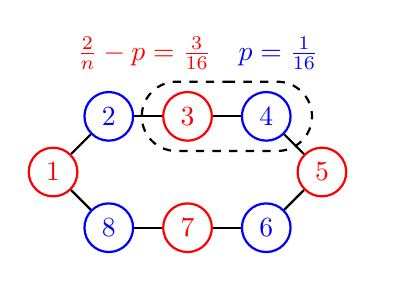
\begin{tikzpicture}[baseline=(current bounding box.north),-,auto,node distance=1cm,
                    thick,main node/.style={circle,draw,font=\sffamily\bfseries}]

  \node[main node,color=red] (1) {$1$};
  \node[main node,color=blue] (2) [above right of=1] {$2$};
  \node[main node,color=red] (3) [right of=2] {$3$};
  \node[main node,color=blue] (4) [right of=3] {$4$};
  \node[main node,color=red] (5) [below right of=4] {$5$};
  \node[main node,color=blue] (6) [below left of=5] {$6$};
  \node[main node,color=red] (7) [left of=6] {$7$};
  \node[main node,color=blue] (8) [left of=7] {$8$};
  

  \path[every node/.style={font=\sffamily}]
  (1) edge (2)
  (2) edge (3)
  (3) edge (4)
  (4) edge (5)
  (5) edge (6)
  (6) edge (7)
  (7) edge (8)
  (8) edge (1);
  
  \node (Box1) [draw,dashed,rounded rectangle,fit=(3) (4)] {};
  
  \node [shift={(-0.4cm,0.8cm)},text width=2cm,color=red] at (3) {$\frac{2}{n}-p=\frac{3}{16}$};
  \node [shift={(0.4cm,0.8cm)},text width=1.5cm,color=blue] at (4) {$p=\frac{1}{16}$};
   
\end{tikzpicture}
\end{center}
\caption{ $C_{8}$ with the \textcolor{blue}{blue nodes being ``even'' nodes} started at with probability $\frac{1}{16}$ and the \textcolor{red}{red nodes being ``odd'' nodes} started at with probability $\frac{3}{16}$.}
\end{examplefigure}

\begin{lemma}
When $n$ and $m$ are both even, following the Alternating Random Hamiltonian Patrol, if feasible, gives the same lower bound as the random Hamiltonian patrol, i.e $V \geq \frac{m}{n}$.
\end{lemma}

\begin{proof}
During any attack interval $I$ which is of even length, then $W(I)$ contains $m'$ ``even'' and $m'$ ``odd'' nodes for a total of $m=2m'$ nodes. Therefore by following the Alternating Random Hamiltonian Patrol, $\pmb{\pi}_{ARHP}$, with probability $p$ at ``even'' nodes and probability $\frac{2}{n}-p$ at ``odd'' nodes. Then

\begin{align*}
&P(\bm{\pi}_{ARHP},[i,I]) \geq \underbrace{\overbrace{p}^{\text{even node}}+\overbrace{\frac{2}{n}-p}^{\text{odd node}}+p+\frac{2}{n}-p+...+p+\frac{2}{n}-p}_{m=2m' \text{ elements}} \\
&=m' p+m'(\frac{2}{n}-p)=\frac{2m'}{n}=\frac{m}{n} \quad \forall i \in N \quad \forall I \subseteq \mathcal{T}
\end{align*}
Hence as it holds for all pure attacks
$$P(\bm{\pi}_{ARHP},\bm{\phi}) \geq \frac{m}{n} \quad \forall \bm{\phi} \in \Phi$$
Hence $V \geq \frac{m}{n}$ .
\end{proof}

If $m$ is odd, say $m=2m'+1$ then in the above we get two possibilities for each node depending on the interval choice either $p+\frac{m-1}{n}$ or $\frac{m+1}{n}-p$. So choosing anything other than $p=\frac{1}{n}$ (which is the Random Hamiltonian Patrol strategy) gives a worse result for the patroller.

While not getting a better lower bound, the ARHP does give some control on how to perform optimally in a Hamiltonian graph. The idea of distributing the probability $\frac{2}{n}$ between two types of nodes can be extended to the idea of distributing the probability $\frac{k}{n}$ between $k$ types of nodes (as seen in appendix \ref{appendix:Hamiltonian Graph}).
\subsection{Star graph solution}
As a special case of Complete bipartite we have the star graph, $S_{n}=K_{1,n}$, that is a tree with one internal node (the centre) and $n$ leaf nodes (the external nodes). Hence $V(S_{n})=V(K_{1,n})=\frac{m}{2n}$ for $m<2n$ (by the Complete bipartite corollary(\ref{Corollary:Complete Bipartite})). This is achieved by the patroller forming a patrol which alternates between different  external nodes and the centre, and the attacker attacking at all the external nodes with equal probability (for a fixed time interval).
\subsection{Extending the star graph}
\subsection{Joining star graphs by centralised connections}

\section{Strategic Patroller with Random Attackers}
In this section we provide further work developed from the literature review in Section \ref{Section:Patrolling games with random attackers}.

\subsection{Deterministic Attack time experiments}
As the theory  works for all bounded attack time distributions, we shall look at the deterministic attack time, using $P(X_{j}=x_{j})=1$, we can note that this does some level of reduction on the state space as costs are only incurred at states with $s_{j}=B_{j}$ or $B_{j}+1$. The cost function reduces to

\begin{align*}
C_{j}(\bm{s},\bm{v},i)=\begin{cases}
c_{j} \lambda_{j} R_{j} + c_{j} v_{j}  \text{ for } s_{j}=B_{j},i \neq j \\ 
c_{j} \lambda_{j} \text{ for } s_{j}=B_{j}+1,i \neq j  \\
0 \text{ Otherwise} \\
\end{cases}
\end{align*}

Looking at the single node problem, we notice that there is no cost to transition to the state $s=B$, so at this point we must decide if we are renew now or renew at $s=B+1$ or never renew at all (If indifferent between $B+1,B+2,....$)

It is curious whether this sudden spike in the cost (and therefore in the resulting index) will cause any issue with the proposed heuristics.

\begin{Huge}
This numerical experiment needs to be done
\end{Huge}


\section{Strategic Patroller with Random Attackers and Local-observations}
\label{Section:Patrolling games with random attackers and local-observations}
We now look at altering the work summarized in Section \ref{Section:Patrolling games with random attackers} to incorporate suspicious behaviour of attackers who arrive while the patroller is present.

\subsection{Altering the problem for instantaneous moving patroller}
As the standard set-up has a patroller moving at unit speed along the edges, they are never really present at a node (even when waiting). As we wish to have the patroller observe some arrivals we shall first alter this assumption to that of an instantaneous moving patrolling. For now we will use the same assumption that attackers who arrive while the patroller is present are caught, however we will soon assume they are smart enough to not start their attack and instantly get caught.

\begin{myfigure}
\begin{center}
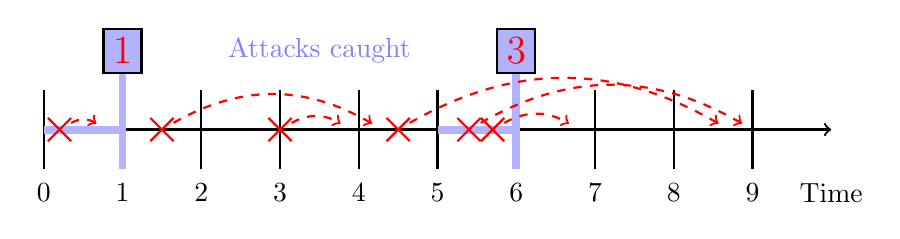
\begin{tikzpicture}[-,auto,node distance=2cm,
                    thick,main node/.style={rectangle,draw,font=\sffamily\Large\bfseries}]

%DRAWING Base line

 \draw[->] (0,0)--(10,0);
 
 \foreach \x in {0,...,9}
 {\draw  (\x,0.5)--(\x,-0.5) ;
  \node (TimeLabel\x) at (\x,-0.8) {$\x$};} 
  
  \node (TimeLabel) at (10,-0.8) {Time};

%Inserting patroller and attackers
  
    \node[main node,fill=blue!30] (Pat1) at (1,1) {\textcolor{red}{$1$}};
  \draw[color=blue!30,line width=0.1cm] (Pat1)--(1,-0.5);
  \draw[color=blue!30,line width=0.1cm] (0,0)--(1,0);
  
  \node[main node,fill=blue!30] (Pat2) at (6,1) {\textcolor{red}{$3$}};
  \draw[color=blue!30,line width=0.1cm] (Pat2)--(6,-0.5);
  \draw[color=blue!30,line width=0.1cm] (5,0)--(6,0);
  
  
  \node[cross=5pt,color=red] (AttackStart1) at (0.2,0) {};
  \node (AttackEnd1) at (0.8,0) {};
  \draw[bend left,color=red,->,dashed] (AttackStart1) to (AttackEnd1);
  
  \node[cross=5pt,color=red] (AttackStart2) at (1.5,0) {};
  \node (AttackEnd2) at (4.3,0) {};
  \draw[bend left,color=red,->,dashed] (AttackStart2) to (AttackEnd2);
  
  \node[cross=5pt,color=red] (AttackStart3) at (3,0) {};
  \node (AttackEnd3) at (3.9,0) {};
  \draw[bend left,color=red,->,dashed] (AttackStart3) to (AttackEnd3);
  
  \node[cross=5pt,color=red] (AttackStart4) at (4.5,0) {};
  \node (AttackEnd4) at (8.7,0) {};
  \draw[bend left,color=red,->,dashed] (AttackStart4) to (AttackEnd4);
  
  \node[cross=5pt,color=red] (AttackStart5) at (5.4,0) {};
  \node (AttackEnd5) at (9,0) {};
  \draw[bend left,color=red,->,dashed] (AttackStart5) to (AttackEnd5);
  
  \node[cross=5pt,color=red] (AttackStart6) at (5.7,0) {};
  \node (AttackEnd6) at (6.8,0) {};
  \draw[bend left,color=red,->,dashed] (AttackStart6) to (AttackEnd6);
  
  
  \node (AttacksCaught) at (3.5,1) {\textcolor{blue!50}{Attacks caught}};
  
       
\end{tikzpicture}
\end{center}
\caption{Example of timing}
\end{myfigure} 

While the standard set-up remains mostly intact, the cost function is slightly altered to accommodate this change. We note there is now a difference in cost depending on if the node is visited or not.

\begin{align*}
C_{j}(\bm{s},i) &= \begin{cases}
0  \text{ if } j=i \\
c_{j} \lambda_{j} \int_{s_{j}-1}^{s_{j}} P(X_{j} \leq t) dt \text{ if } j \neq i \\
\end{cases}
\end{align*}

This change does not the theory that much, the problem can still be reduced to the single node version of the problem. However there is a slight change here, which results in a slight change to the optimal solution and hence the index which is suggested.

The following are the changes

\begin{align*}
&f(k) \equiv \frac{c \lambda \int_{0}^{k-1} P(X \leq t) dt + \omega}{k} \\
&W(k) \equiv c \lambda \left( \int_{k-1}^{k} P(X \leq t) dt - \int_{0}^{k-1} P(X \leq t) dt \right)
\end{align*}

\begin{note}
$W(0)=0$ and for $k \geq B+1$ $W(k)= c \lambda E[X]$
\end{note}

Using this new definition of $W(k)$, Theorem \ref{Theorem:Single node optimal policy} still holds and gives us the optimal policy. Hence suggesting an index of

\begin{align*}
W_{i}(\bm{s}) \equiv c_{i} \lambda_{i} \left( \int_{s_{i}-1}^{s_{i}} P(X_{i} \leq t) dt - \int_{0}^{s_{i}-1} P(X_{i} \leq t) dt \right)
\end{align*}

For completness sake, we provide numerical results for the IRH and IPH defined as before, but using this index.

\subsection{Numerical results for instantaneously moving patroller}
For completeness sake, we provide numerical results for the IRH and IPH defined as before, but using this index.


\begin{huge}
THIS NEEDS TO BE DONE
\end{huge}



\subsection{Altering problem to accommodate local-observable information}
Now that we have established a instantaneously moving patroller, we now introduce the idea of local-observations, that is the patroller witnesses attackers arriving at there current node, but the attackers do not begin there attack immediately,as they are aware of the patroller's presence. For now we assume that any such attacker is only able to delay their attack to start at the beginning of the next time period.

\begin{figure}
\begin{center}
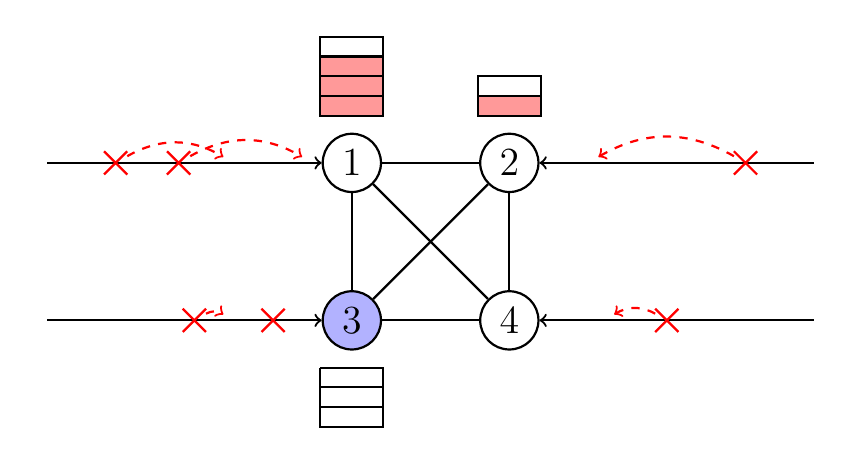
\begin{tikzpicture}[-,auto,node distance=2cm,
                    thick,main node/.style={circle,fill=white,draw,font=\sffamily\Large\bfseries}]

%DRAWING GRAPH
  \node[main node] (1) {$1$};
  \node[main node] (2) [right of=1] {$2$};
  \node[main node,fill=blue!30] (3) [below of=1]  {$3$};
  \node[main node] (4) [below of=2]  {$4$};

  \path[every node/.style={font=\sffamily}]
    (1) edge (2)
        edge (3)
        edge (4)
    (2) edge (3)
        edge (4)
    (3) edge (4);
  
  
%DRAWING ARRIVALS  
  \node (1ArrowStart) [shift={(-4,0)}] at (1) {};
  \draw[->] (1ArrowStart)--(1);
  
  \node[cross=5pt,color=red] (1Cross1) [shift={(-3,0)}] at (1) { };
  \node (1CrossEnd1) [shift={(-1.5,0)}] at (1) {};
  \draw[->,bend left,dashed,color=red] (1Cross1) to (1CrossEnd1);
  \node[cross=5pt,color=red] (1Cross2) [shift={(-2.2,0)}] at (1) { };
  \node (1CrossEnd2) [shift={(-0.5,0)}] at (1) {};
  \draw[->,bend left,dashed,color=red] (1Cross2) to (1CrossEnd2);
  
  \node (2ArrowStart) [shift={(4,0)}] at (2) {};
  \draw[->] (2ArrowStart)--(2);
  
  \node[cross=5pt,color=red] (2Cross1) [shift={(3,0)}] at (2) { };
  \node (2CrossEnd1) [shift={(1,0)}] at (2) {};
  \draw[->,bend right,dashed,color=red] (2Cross1) to (2CrossEnd1);

  \node (3ArrowStart) [shift={(-4,0)}] at (3) {};
  \draw[->] (3ArrowStart)--(3);
  
  \node[cross=5pt,color=red] (3Cross1) [shift={(-2,0)}] at (3) { };
  \node (3CrossEnd1) [shift={(-1.5,0)}] at (3) {};
  \draw[->,bend left,dashed,color=red] (3Cross1) to (3CrossEnd1);
  \node[cross=5pt,color=red] (3Cross1) [shift={(-1,0)}] at (3) { };
  
  \node (4ArrowStart) [shift={(4,0)}] at (4) {};
  \draw[->] (4ArrowStart)--(4);
  
  \node[cross=5pt,color=red] (4Cross1) [shift={(2,0)}] at (4) { };
  \node (4CrossEnd1) [shift={(1.2,0)}] at (4) {};
  \draw[->,bend right,dashed,color=red] (4Cross1) to (4CrossEnd1);
  
%Drawing Observable capacity boxes
 \node (1LowerLeft) [shift={(-0.4,0.6)}] at (1) { };
 \node (1LowerRight) [shift={(0.4,0.6)}] at (1) { };
 \node (1UpperLeft) [shift={(-0.4,1.6)}] at (1) { };
 \node (1UpperRight) [shift={(0.4,1.6)}] at (1) { }; 
 
 \draw[-] (1LowerLeft.center)--(1LowerRight.center)--(1UpperRight.center)
 --(1UpperLeft.center)--(1LowerLeft.center);
 
 \node (1FillPointLeft1) [shift={(0,0.25)}] at (1LowerLeft) { };
 \node (1FillPointRight1) [shift={(0,0.25)}] at (1LowerRight) { };
 \node (1FillPointLeft2) [shift={(0,0.5)}] at (1LowerLeft) { };
 \node (1FillPointRight2) [shift={(0,0.5)}] at (1LowerRight) { };
 \node (1FillPointLeft3) [shift={(0,0.75)}] at (1LowerLeft) { };
 \node (1FillPointRight3) [shift={(0,0.75)}] at (1LowerRight) { };

 \filldraw[fill=red!40!white, draw=black] (1LowerLeft) rectangle (1FillPointRight3);
 
 \draw[-] (1FillPointLeft1.center)--(1FillPointRight1.center);
 \draw[-] (1FillPointLeft2.center)--(1FillPointRight2.center);
 \draw[-] (1FillPointLeft3.center)--(1FillPointRight3.center);
 
 
 
 \node (2LowerLeft) [shift={(-0.4,0.6)}] at (2) { };
 \node (2LowerRight) [shift={(0.4,0.6)}] at (2) { };
 \node (2UpperLeft) [shift={(-0.4,1.1)}] at (2) { };
 \node (2UpperRight) [shift={(0.4,1.1)}] at (2) { }; 
 
 \draw[-] (2LowerLeft.center)--(2LowerRight.center)--(2UpperRight.center)
 --(2UpperLeft.center)--(2LowerLeft.center);
 
 \node (2FillPointLeft1) [shift={(0,0.25)}] at (2LowerLeft) { };
 \node (2FillPointRight1) [shift={(0,0.25)}] at (2LowerRight) { };

 \filldraw[fill=red!40!white, draw=black] (2LowerLeft) rectangle (2FillPointRight1);
 
 \draw[-] (1FillPointLeft1.center)--(1FillPointRight1.center);
 
 
 \node (3LowerLeft) [shift={(-0.4,-0.6)}] at (3) { };
 \node (3LowerRight) [shift={(0.4,-0.6)}] at (3) { };
 \node (3UpperLeft) [shift={(-0.4,-1.35)}] at (3) { };
 \node (3UpperRight) [shift={(0.4,-1.35)}] at (3) { }; 
 
 \draw[-] (3LowerLeft.center)--(3LowerRight.center)--(3UpperRight.center)
 --(3UpperLeft.center)--(3LowerLeft.center);
 
 \node (3FillPointLeft1) [shift={(0,-0.25)}] at (3LowerLeft) { };
 \node (3FillPointRight1) [shift={(0,-0.25)}] at (3LowerRight) { };
 \node (3FillPointLeft2) [shift={(0,-0.5)}] at (3LowerLeft) { };
 \node (3FillPointRight2) [shift={(0,-0.5)}] at (3LowerRight) { };

 
 \draw[-] (3FillPointLeft1.center)--(3FillPointRight1.center);
 \draw[-] (3FillPointLeft2.center)--(3FillPointRight2.center);
    
\end{tikzpicture}
\end{center}
\caption{Example of $G=(K_{4},\bm{X},\bm{b},\bm{\lambda},\bm{c})$ with patroller currently at node $3$}
\end{figure}


\begin{myfigure}
\begin{center}
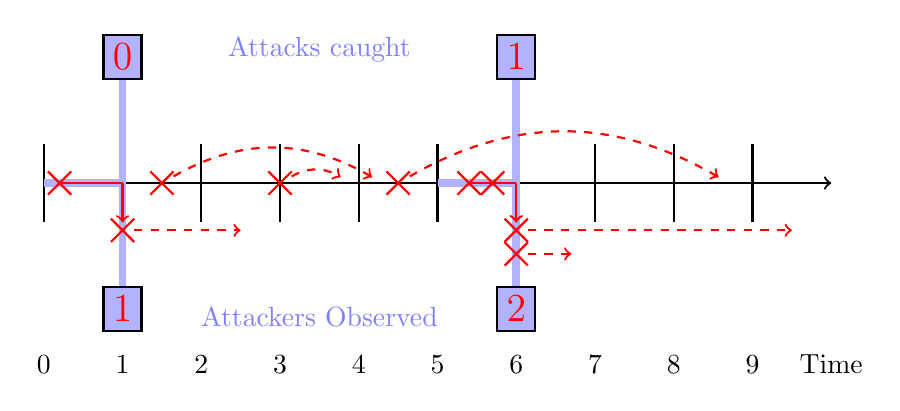
\begin{tikzpicture}[-,auto,node distance=2cm,
                    thick,main node/.style={rectangle,draw,font=\sffamily\Large\bfseries}]

%DRAWING Base line

 \draw[->] (0,0)--(10,0);
 
 \foreach \x in {0,...,9}
 {\draw  (\x,0.5)--(\x,-0.5) ;
  \node (TimeLabel\x) at (\x,-2.3) {$\x$};} 
  
  \node (TimeLabel) at (10,-2.3) {Time};

%Inserting patroller and attackers
  \node[main node,fill=blue!30] (Pat1) at (1,1.6) {\textcolor{red}{$0$}};
  \node[main node,fill=blue!30] (PatObs1) at (1,-1.6) {\textcolor{red}{$1$}};
  \draw[color=blue!30,line width=0.1cm] (Pat1)--(PatObs1);
  \draw[color=blue!30,line width=0.1cm] (0,0)--(1,0);
  
  \node[main node,fill=blue!30] (Pat2) at (6,1.6) {\textcolor{red}{$1$}};
  \node[main node,fill=blue!30] (PatObs2) at (6,-1.6) {\textcolor{red}{$2$}};
  \draw[color=blue!30,line width=0.1cm] (Pat2)--(PatObs2);
  \draw[color=blue!30,line width=0.1cm] (5,0)--(6,0);
  
  
  \node[cross=5pt,color=red] (AttackStart1) at (0.2,0) {};
  \draw[-,color=red] (AttackStart1.center) to (1,0);
  \draw[->,color=red] (1,0) to (1,-0.5);
  \node[cross=5pt,color=red] (NewAttackStart1) at (1,-0.6) {};
  \draw[->,color=red,dashed] (NewAttackStart1) to (2.5,-0.6);
  
  \node[cross=5pt,color=red] (AttackStart2) at (1.5,0) {};
  \node (AttackEnd2) at (4.3,0) {};
  \draw[bend left,color=red,->,dashed] (AttackStart2) to (AttackEnd2);
  
  \node[cross=5pt,color=red] (AttackStart3) at (3,0) {};
  \node (AttackEnd3) at (3.9,0) {};
  \draw[bend left,color=red,->,dashed] (AttackStart3) to (AttackEnd3);
  
  \node[cross=5pt,color=red] (AttackStart4) at (4.5,0) {};
  \node (AttackEnd4) at (8.7,0) {};
  \draw[bend left,color=red,->,dashed] (AttackStart4) to (AttackEnd4);
  
  \node[cross=5pt,color=red] (AttackStart5) at (5.4,0) {};
  \draw[-,color=red] (AttackStart5.center) to (6,0);
  \draw[->,color=red] (6,0) to (6,-0.5);
  \node[cross=5pt,color=red] (NewAttackStart5) at (6,-0.6) {};
  \draw[->,color=red,dashed] (NewAttackStart5) to (9.5,-0.6);
  
  
  \node[cross=5pt,color=red] (AttackStart6) at (5.7,0) {};
  \draw[-,color=red] (AttackStart6.center) to (6,0);
  \draw[->,color=red] (6,0) to (6,-0.5);
  \node[cross=5pt,color=red] (NewAttackStart5) at (6,-0.9) {};
  \draw[->,color=red,dashed] (NewAttackStart5) to (6.7,-0.9);

 \node (AttacksCaught) at (3.5,1.7) {\textcolor{blue!50}{Attacks caught}};
 
 \node (AttacksObs) at (3.5,-1.7) {\textcolor{blue!50}{Attackers Observed}};
  
       
\end{tikzpicture}
\end{center}
\caption{Example of timing}
\end{myfigure}

The problem can still be formulated as a MDP, however our states now need to hold the information about how many attackers where observed when the node was last visited. Our state space is

$$\Omega= \{ (\bm{s},\bm{v})=(s_{1},...,s_{n},v_{1},...,v_{n}) \, | \, s_{i}=1,2,...., \; v_{i}=0,1,...  \text{ for } i=1,...,n\}$$

Where as before, $s_{i}$ denotes the time since the last decision to visit node $i$ was taken and the newly introduced $v_{i}$ denotes how many attackers where observed when the patroller last visited node $i$.The current node is $l(\bm{s},\bm{v})=\argmin_{i} s_{i}$ and the decisions from $(\bm{s},\bm{v})$ are still adjacent node, $\mathcal{A}(\bm{s},\bm{v})$. The transition when node $i$ is chosen to move to are $\phi(\bm{s},\bm{v},i)=(\widetilde{\bm{s}},\widetilde{\bm{v}})$, where; $\widetilde{s}_{i}=1$,  $\widetilde{s}_{j}=s_{j}+1 \; \forall j \neq i$, $\widetilde{v}_{i} \sim Po(\lambda_{i})$ and $\widetilde{v}_{j}=v_{j} \; \forall j \neq i$.

That is the $\bm{s}$ state transitions as before, and the $\bm{v}$ state updates the chosen node to be the amount observed while the patroller is at the node, which is drawn from a Poisson distribution of rate $\lambda_{i}$ due to the arrivals being a Poisson Process.

Again the future of the process is independent of its past, so we can formulate its movement as an MC and hence the patrollers problem is a MDP.

The patroller incurs cost $c_{j}$ for all successful attacks at node $j$. A successful attack will fall into two categories; an observed attack or an attacker who arrived. We simply sum the expected costs of both types of attacker to work out the cost at a node for the next unit time, given we choose to move to node $i$.

\begin{align*}
C_{j}(\bm{s},i) &= \begin{cases}
0  \text{ if } j=i \\
\underbrace{c_{j} P(s_{j}-1 < X_{j} \leq s_{j})}_{\text{Observed finishing}} + \underbrace{c_{j} \lambda_{j} \int_{s_{j}-1}^{s_{j}} P(X_{j} \leq t) dt}_{\text{Arrivals finishing}} \text{ if } j \neq i \\
\end{cases}
\end{align*}

We run into the same problem as before, with a countably infinite state space, $\Omega$, we therefore wish to bound ourselves to a finite state space. As before we can bound the attack times, defining $B_{j}$ as in \ref{Equation:Definition of attack time bound}, but this only partially solves our problem, as it bounds the $\bm{s}$ part of the state space but not the $\bm{v}$ part.

To bound $\bm{v}$ we introduce a observable capacity, $\bm{b}$, where $b_{i}$ is the maximum number of local-observations at node $i$. We assume that all other attackers fail once this capacity is reached.

\begin{figure}[H]
\begin{center}
\resizebox{0.8\linewidth}{!}{
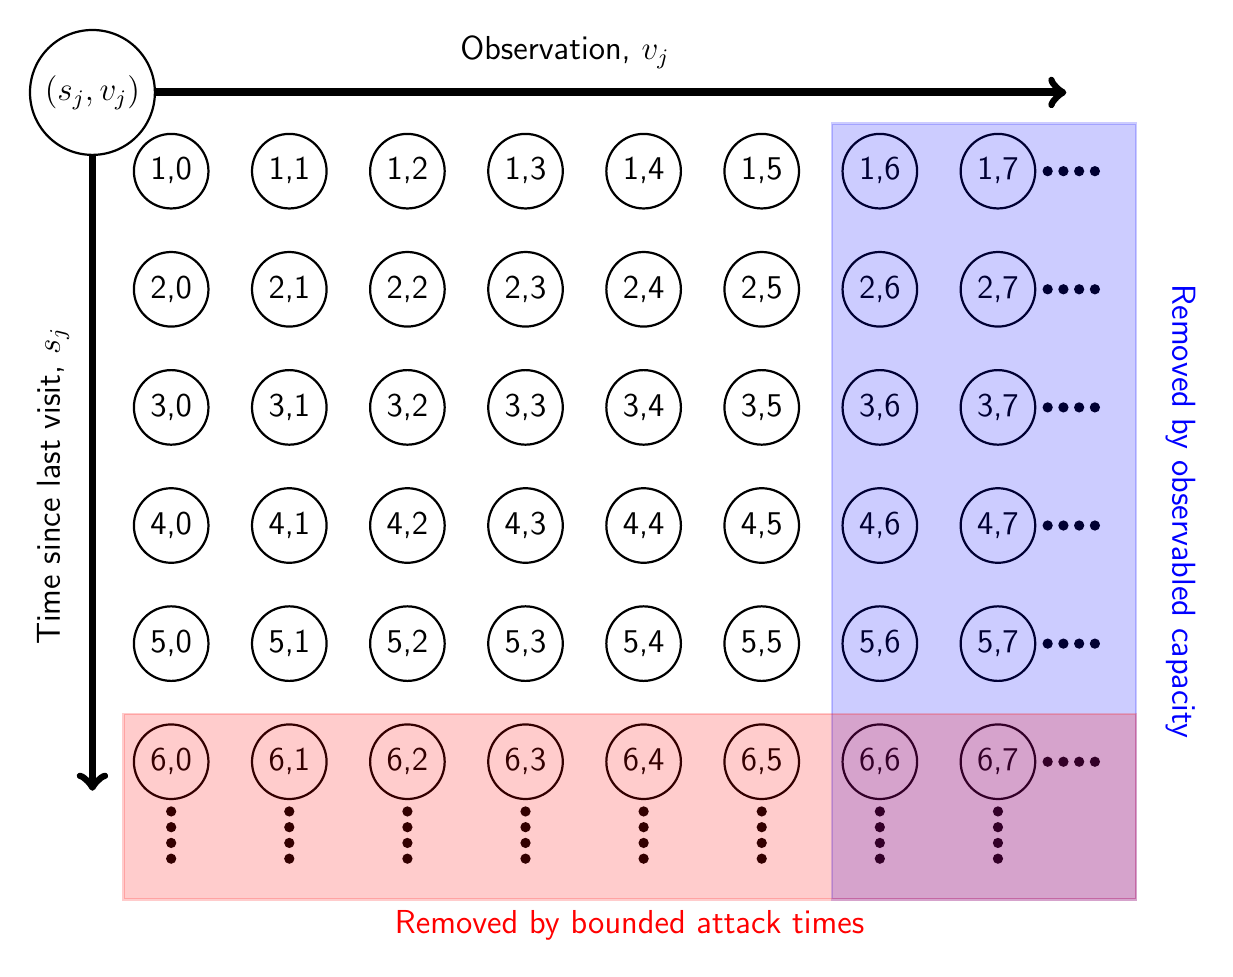
\begin{tikzpicture}[-,auto,node distance=1cm,
                    thick,main node/.style={circle,fill=white,draw,font=\sffamily\large,minimum size=0.5cm}]
 \foreach \x in {0,...,7}
    \foreach \y in {0,...,5} 
       {\pgfmathtruncatemacro{\label}{\x - 5 *  \y +21}
        \pgfmathtruncatemacro{\v}{\x}
        \pgfmathtruncatemacro{\s}{6-\y}
       \node [main node]  (\x\y) at (1.5*\x,1.5*\y) {\s,\v};} 

\node (XaxisLeft) [shift={(-0.5,1)}] at (05) {};
\node (XaxisRight) [shift={(1,1)}] at (75) {};

\node (YaxisBottom) [shift={(-1,-0.5)}] at (00) {};
\node (YaxisTop) [shift={(-1,1)}] at (05) {};

\draw[->,line width=1mm] (XaxisLeft)--(XaxisRight);
\draw[->,line width=1mm] (YaxisTop)--(YaxisBottom);

\node[font=\sffamily\large] (OLabel) [shift={(0.5,1.5)}] at (35) {Observation, $v_{j}$};
\node[font=\sffamily\large] (SLabel) [shift={(-1.5,0.5)}] at (02) {\rotatebox{90}{Time since last visit, $s_{j}$}};

\node[main node] (Example) [shift={(-1,1)}] at (05) {$(s_{j},v_{j})$};

\foreach \y in {0,...,5}
{\node (DottedStart\y) [shift={(0.5,0)}] at (7\y) {};
 \node (DottedEnd\y) [shift={(1.5,0)}] at (7\y) {};
 \draw[decorate sep={1mm}{2mm},fill] (DottedStart\y)--(DottedEnd\y);}
 
\foreach \x in {0,...,7}
{\node (\x DottedStart) [shift={(0,-0.5)}] at (\x0) {};
 \node (\x DottedEnd) [shift={(0,-1.5)}] at (\x0) {};
 \draw[decorate sep={1mm}{2mm},fill] (\x DottedStart)--(\x DottedEnd);
}

\node (Box1) [draw,thick,fit=(65) (60) (DottedEnd5) (DottedEnd0) (6DottedEnd) (7DottedEnd),fill,blue,opacity=0.2] {};

\node (Box2) [draw,thick,fit=(00) (70)(DottedEnd0) (0DottedEnd) (7DottedEnd),fill,red,opacity=0.2] {};

\node[font=\sffamily\large,color=blue] (Box1Text) [shift={(2.5,0)}] at (Box1) {\rotatebox{270}{Removed by observabled capacity}};

\node[font=\sffamily\large,color=red] (Box2Text) [shift={(0,-1.5)}] at (Box2) {Removed by bounded attack times};           

\end{tikzpicture}
}
\end{center}
\caption{State space diagram for node $j$, with \textcolor{blue}{$b_{j}=5$} and \textcolor{red}{$B_{j}=4$} (e.g. $X_{j} \leq 3.7$)}
\end{figure}

This change to a finite state space, $\Omega = \{ (\bm{s},\bm{v})=(s_{1},...,s_{n},v_{1},...,v_{n}) \, | \, s_{i}=1,2,....,B_{i}+1 \; v_{i}=0,1,...,b_{i}  \text{ for } i=1,...,n\}$ and caps the transitions. That is that $\widetilde{s}_{j}= \min \{s_{j}+1, B_{j}+1 \}$ and $\widetilde{v}_{i} \sim TPo(\lambda_{i},b_{i)}$, where $TPo(\lambda,b)$ is the truncated Poisson distribution, with all the tail probability at the value $b_{i}$. I.e.

\begin{align*}
P(TPo(\lambda,b)=\begin{cases}
P(Po(\lambda) \text{ if } i \neq b \\
P(Po(\lambda) \geq i) \text{ if } i=b \\
0 \text{ Otherwise}
\end{cases}
\end{align*}

Even though the state space is now finite, the transitions are not deterministic, so a cyclic behaviour is not induced when the same state is reached again. For notational purposes we will still use $\phi^{k}_{\pi}(\bm{s}_{0},\bm{v}_{0})$ to be the state after $k$ transitions from $(\bm{s}_{0},\bm{v}_{0})$.

\begin{Huge}
More work is needed to see if the cyclic behaviour property does still hold just in some probabilistic fashion
\end{Huge}

This problem, as before, can be solved by standard techniques such as value iteration or linear programing to compute the long-run average cost. This is left to Appendix \ref{Appendix:Optimal Solution for Random Attacker with Local-Observations}.

We can then use the standard reduction tools of making the problem into a MN problem and then applying the TR constraint and/or the Lagrangian relaxation. We shall therefore focus on the Lagrangian relaxation which is equivalent to the single node problem.

That is we wish to minimize $V(\pi)+\omega \mu(\pi)$. Our state space is more complicated than before due to the inclusion of the time since it was last visited and the amount of local-observations made when it was last visited.

\subsection{Deterministic attack time assumption}
Because our state space is hard to deal with,in the single node problem, we shall reduce the problem, by assuming that the attack times are deterministic, that is $P(X=x)=1$, this reduces our cost function to

\begin{align*}
C_{j}(\bm{s},\bm{v},i)=\begin{cases}
c_{j} \lambda_{j} R_{j} + c_{j} v_{j}  \text{ for } s_{j}=B_{j},i \neq j \\ 
c_{j} \lambda_{j} \text{ for } s_{j}=B_{j}+1,i \neq j  \\
0 \text{ Otherwise} \\
\end{cases}
\end{align*}
Where $R_{j}=B_{j}-x_{j}$. We see that we only worry about incurring costs in states when $s_{i}=B_{i}$ or $B_{i}+1$ for some $i$.


\subsection{Single node solution}
\subsection{Indices, heuristics and numerical experiments}

\section{Future Work}
\subsection{Proof completions}
\subsection{Extending Discrete Attack time to generic distributions}
\subsection{Strategic Patroller with Random Attackers on Edges}

%End of main part of document
\bibliography{mybib}

\newpage
\appendix
\pagenumbering{roman}
\appendixpage
\addappheadtotoc
\section{Graph Definitions}
\label{Appendix:Graph Definitions}
\begin{definition}[Graph]
A \textit{graph}, $G=G(N,E)$, is made up of: a set of \textit{nodes} (also called \textit{vertices} or \textit{points}), $N$, which are places ; and a set of \textit{edges} (also called \textit{arcs} or lines), $E$, which are connections between places, so elements of $E$ must be two-element subsets of $N$.
\end{definition}


\begin{definition}[Subgraph]
A graph $Q'=(N',E')$ is said to be a \textit{subgraph} of $Q=(N,E)$ if $N' \subset N$ and $E' \subset E$.

A subgraph is said to be \textit{induced} by $N'$ (or \textit{edge-preserving}) if $E'$ contains all edges (from $E$) that have both end points in $N'$.
\end{definition}


\begin{myfigure}
\begin{center}
\begin{submyfigure}{.3\textwidth}
\begin{center}
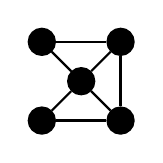
\begin{tikzpicture}[baseline=(current bounding box.north),-,auto,node distance=1cm,
                    thick,main node/.style={circle,draw,fill,font=\sffamily\bfseries}]

  \node[main node] (1) {};
  \node[main node] (2) [right of=1] {};
  \node[main node] (3) [shift={(0.5,-0.5)}] at (1) {};
  \node[main node] (4) [below of=1] {};
  \node[main node] (5) [below of=2] {};
  

  \path[every node/.style={font=\sffamily}]
    (1) edge  (2)
        edge  (3)
    (2) edge  (3)
        edge  (5)
    (4) edge  (3)
        edge  (5)
    (5) edge  (3);
                        
\end{tikzpicture}
\end{center}
\caption{$Q$}
\label{subexamplefigure: before subgraphs}
\end{submyfigure}
\begin{submyfigure}{.3\textwidth}
\begin{center}
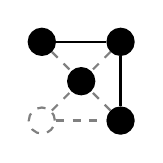
\begin{tikzpicture}[baseline=(current bounding box.north),-,auto,node distance=1cm,
                    thick,main node/.style={circle,draw,fill,font=\sffamily\bfseries}, alt node/.style={circle,draw,dashed,gray,font=\sffamily\bfseries}]

  \node[main node] (1) {};
  \node[main node] (2) [right of=1] {};
  \node[main node] (3) [shift={(0.5,-0.5)}] at (1) {};
  \node[alt node] (4) [below of=1] {};
  \node[main node] (5) [below of=2] {};
  

  \path[every node/.style={font=\sffamily}]
    (1) edge  (2)
    (2) edge  (5);
    
  \path[dashed,gray,font=\sffamily]
    (1) edge (3)
    (2) edge (3)
    (4) edge (3)
        edge (5)
    (5) edge (3);          
                        
\end{tikzpicture}
\end{center}
\caption{$Q_{1}$}
\label{subexamplefigure: subgraph}
\end{submyfigure}
\begin{submyfigure}{.3\textwidth}
\begin{center}
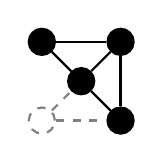
\begin{tikzpicture}[baseline=(current bounding box.north),-,auto,node distance=1cm,
                    thick,main node/.style={circle,draw,fill,font=\sffamily\bfseries}, alt node/.style={circle,draw,dashed,gray,font=\sffamily\bfseries}]

  \node[main node] (1) {};
  \node[main node] (2) [right of=1] {};
  \node[main node] (3) [shift={(0.5,-0.5)}] at (1) {};
  \node[alt node] (4) [below of=1] {};
  \node[main node] (5) [below of=2] {};
  

  \path[every node/.style={font=\sffamily}]
    (1) edge  (2)
    (2) edge  (5)
    (1) edge (3)
    (2) edge (3)
    (5) edge (3);
    
  \path[dashed,gray,font=\sffamily]
    (4) edge (3)
        edge (5);          
                        
\end{tikzpicture}
\end{center}
\caption{$Q_{1}$}
\label{subexamplefigure: induced subgraph}
\end{submyfigure}
\caption{ $Q_{1}$ is a subgraph of $Q$. However it is not induced as it is missing possible edges connecting nodes that existed in $Q$. $Q_{2}$ shows the induced subgraph on the chosen set of nodes. }
\end{center}
\label{examplefigure: subgraph example}
\end{myfigure}

\begin{definition}[Walk,Path,Trail,Cycle]
A sequence of nodes $(n_{0},n_{1},...,n_{l})$ is a \textit{walk} of length $l$ if $e_{n_{i},n_{i+1}} \in E$ $\forall i=0,...,l-1$. Corresponding to a walk is the sequnece of $l$ edges $(e_{n_{0},n_{1}},e_{n_{1},n_{2}},...,e_{n_{l-1},n_{l}})$.

A walk becomes a trail if each edge in the walk is distinct, i.e $e_{n_{i},n_{i+1}} \neq e_{n_{j},n_{j+1}} \forall i \neq j$. A trail becomes a path if each node in the walk is distinct (except possibly the start and final node), i.e $n_{i} \neq n_{j} \forall i \forall i < j \geq l-1$.

A walk,trail or path is said to be \textit{closed} if the start and end nodes are the same. A \textit{cycle} is a closed path with length, $l \geq 3$ (with the special case of $l=3$ being called a \textit{triangle}).
\end{definition}

\begin{definition}[Hamiltonian cycle]
A \textit{Hamiltonian cycle} is a cycle which contains every node on the graph, i.e it is a cycle of length $l=|N|$. A graph that exhibits a Hamiltonian cycle is called \textit{Hamiltonian}
\end{definition}

\begin{figure}
\begin{center}
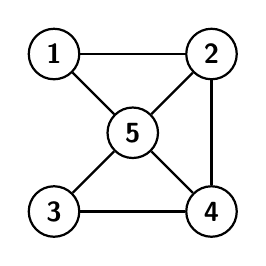
\begin{tikzpicture}[baseline=(current bounding box.north),-,auto,node distance=2cm,
                    thick,main node/.style={circle,draw,font=\sffamily\bfseries}]

  \node[main node] (1) {1};
  \node[main node] (2) [right of=1] {2};
  \node[main node] (3) [shift={(1,-1)}] at (1) {5};
  \node[main node] (4) [below of=1] {3};
  \node[main node] (5) [below of=2] {4};
  

  \path[every node/.style={font=\sffamily}]
    (1) edge  (2)
        edge  (3)
    (2) edge  (3)
        edge  (5)
    (4) edge  (3)
        edge  (5)
    (5) edge  (3);
                        
\end{tikzpicture}
\end{center}
\caption{Graph, $Q$}
\label{figure: walks on graph Q}
\end{figure}

\begin{example}
For the graph $Q$ as in Figure \ref{figure: walks on graph Q}:
\begin{itemize}
\item An example of a walk is $(1,2,1,5,4,2)$
\item An example of a trail is $(1,2,5,3,4,5,1)$
\item An example of a path is $(1,2,4,3)$
\item An example of a Hamiltonian cycle is $(1,2,4,3,5,1)$
\end{itemize}
Hence we would call the graph $Q$ Hamiltonian.
\end{example}

\begin{definition}[Complete graphs]
The \textit{complete graph}, $K_{n}$, is a graph of $n$ nodes, in which all edges are present, i.e $e_{i,i'} \in E \; \forall i,i' \in N$.
\end{definition}

\begin{myfigure}
\begin{center}
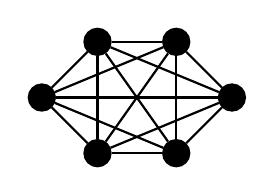
\begin{tikzpicture}[baseline=(current bounding box.north),-,auto,node distance=1cm,
                    thick,main node/.style={circle,fill,draw,font=\sffamily\bfseries}]

  \node[main node] (1) {};
  \node[main node] (2) [right of=1] {};
  \node[main node] (3) [below left of=1] {};
  \node[main node] (4) [below right of=2] {};
  \node[main node] (5) [below right of=3] {};
  \node[main node] (6) [below left of=4] {};
  

  \path[every node/.style={font=\sffamily}]
    (1) edge  (2)
        edge  (3)
        edge  (4)
        edge  (5)
        edge  (6)
    (2) 
        edge  (3)
        edge  (4)
        edge  (5)
        edge  (6)
    (3) 
        edge  (4)
        edge  (5)
        edge  (6)
    (4) edge  (5)
        edge  (6)
    (5) edge  (6);        
                     
\end{tikzpicture}
\caption{The complete graph of $6$ nodes,$K_{6}$.}
\end{center}
\end{myfigure}

\begin{definition}[Bipartite]
A graph is said to be \textit{bipartite} if $N=A \cup B$, where $A \cap B= \emptyset$ ,and $e_{i,i'} \notin E \, \forall i,i' \in A$, $e_{i,i'} \notin E \, \forall i,i' \in B$.
\end{definition}

\begin{definition}[Complete bipartite]
The \textit{complete biparite graph}, $K_{a,b}$, is a bipartite graph of $a+b$ nodes (where $|A|=a$,$|B|=b$), in which all edges are present, i.e $e_{i,i'} \in E \; \forall i \in A \, \forall i' \in B$ and $e_{i,i'} \in E \; \forall i \in B \, \forall i' \in A$.
\end{definition}

\begin{myfigure}
\begin{center}
\begin{submyfigure}{.45\textwidth}
\begin{center}
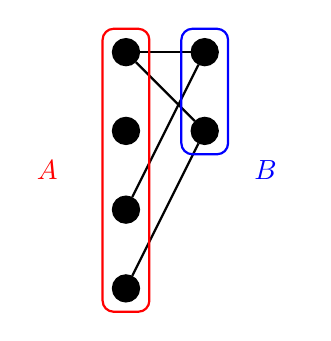
\begin{tikzpicture}[baseline=(current bounding box.north),-,auto,node distance=1cm,
                    thick,main node/.style={circle,draw,fill,font=\sffamily\bfseries}]

  \node[main node] (1) {};
  \node[main node] (2) [below of=1] {};
  \node[main node] (3) [below of=2] {};
  \node[main node] (4) [below of=3] {};
  \node[main node] (5) [right of=1] {};
  \node[main node] (6) [below of=5] {};
  

  \path[every node/.style={font=\sffamily}]
    (1) edge  (5)
        edge  (6)
    (3) edge  (5)
    (4) edge  (6);
        
  \node (ABox) [draw,rounded corners,red, fit= (1) (2) (3) (4)] {};
  \node (BBox) [draw,rounded corners,blue, fit= (5) (6)] {};
  
  \node [left=0.5cm,text width=0.5cm,red] at (ABox) {$A$};
  \node [right=1.5cm,text width=0.5cm,blue] at (ABox) {$B$};              
                     
\end{tikzpicture}
\end{center}
\caption{$Q$}
\label{subfigure: bipartite Q}
\end{submyfigure}
\begin{submyfigure}{.45\textwidth}
\begin{center}
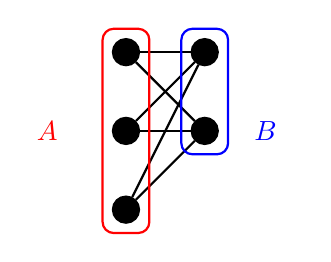
\begin{tikzpicture}[baseline=(current bounding box.north),-,auto,node distance=1cm,
                    thick,main node/.style={circle,draw,fill,font=\sffamily\bfseries}]

  \node[main node] (1) {};
  \node[main node] (2) [below of=1] {};
  \node[main node] (3) [below of=2] {};
  \node[main node] (4) [right of=1] {};
  \node[main node] (5) [below of=4] {};
  

  \path[every node/.style={font=\sffamily}]
    (1) edge  (4)
        edge  (5)
    (2) edge  (4)
        edge  (5)
    (3) edge  (4)
        edge  (5);
        
  \node (ABox) [draw,rounded corners,red, fit= (1) (2) (3)] {};
  \node (BBox) [draw,rounded corners,blue, fit= (4) (5)] {};
  
  \node [left=0.5cm,text width=0.5cm,red] at (ABox) {$A$};
  \node [right=1.5cm,text width=0.5cm,blue] at (ABox) {$B$};              
                     
\end{tikzpicture}
\end{center}
\caption{$K_{3,2}$}
\label{subfigure: complete bipartite}
\end{submyfigure}
\caption{ \ref{subfigure: bipartite Q} is an example of a bipartite graph, Q. \ref{subfigure: complete bipartite} is the complete bipartite graph with set sizes of $3$ and $2$.}
\end{center}
\end{myfigure}

\begin{definition}[Subdivision,Smoothing]
A \textit{Subdivision} (or \textit{expansion}) of a graph, $G$, is a new graph $G'$ which is made by subdividing a chosen edge. The subdivision of an edge $\{u,v\}$ yields a graph with a new node $w$ and the splitting of the edge $\{u,v\}$ into $\{u,w\}$ and $\{w,v\}$.

The reverse process is called \textit{Smoothing} of a graph, $G$, is a new graph $G'$ which is made by smoothing between two nodes. The smoothing out of a node pair $(u,v)$, with $d(u,v)=2$ and with $w$ between them, then $w$ is removed along with the edges $\{u,w\}$ and $\{v,w\}$, then the edge $\{u,v\}$ is placed to connect $u$ and $v$. 
\end{definition}

\begin{myfigure}
\begin{center}
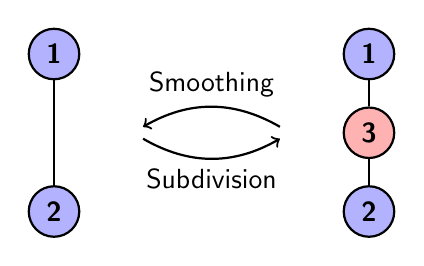
\begin{tikzpicture}[baseline=(current bounding box.north),-,auto,node distance=2cm,
                    thick,main node/.style={circle,draw,font=\sffamily\bfseries}]

  \node[main node,fill=blue!30] (1) {1};
  \node[main node,fill=blue!30] (2) [below of=1] {2};
  

  \path[every node/.style={font=\sffamily}]
    (1) edge  (2);
    
  \node (AP1) [shift={(1,-1)}] {};
  \node (AP2) [shift={(3,-1)}] {};
  
  \path[->,bend right,every node/.style={font=\sffamily}]
    (AP1) edge node[below] {Subdivision} (AP2)
    (AP2) edge node[above] {Smoothing} (AP1);
      
  
  \node[main node,fill=blue!30] (3) [shift={(4,0)}]{1};
  \node[main node,fill=red!30] (4) [shift={(4,-1)}]{3};
  \node[main node,fill=blue!30] (5) [shift={(4,-2)}]{2};
  
  \path[every node/.style={font=\sffamily}]
    (3) edge  (4)
    (4) edge  (5);
  
    
                        
\end{tikzpicture}
\caption{Subdivision and Smoothing of the edge $\{1,2\}$}
\end{center}
\end{myfigure}

\section{Optimal Solution for a Random Attacker}
\label{Appendix:Optimal Solution for a Random Attacker}

\section{Optimal Solution for Random Attacker with Local-Observations}
\label{Appendix:Optimal Solution for Random Attacker with Local-Observations}
\end{document}
